\documentclass[11pt, a4paper]{article}

% --- Tipografía y Lenguaje ---
\usepackage[T1]{fontenc}
\usepackage[utf8]{inputenc}
\usepackage[spanish, es-tabla]{babel}
\usepackage{lmodern}
\usepackage{microtype}
\usepackage{graphicx}
\decimalpoint

% --- Matemáticas ---
\usepackage{amsmath, amssymb, amsfonts, bm} % 'bm' para negritas en símbolos matemáticos

% --- Formato de Página y Encabezados ---
\usepackage[top=2.5cm, bottom=2.5cm, left=2cm, right=2cm]{geometry}
\usepackage{fancyhdr}
\pagestyle{fancy}
\fancyhf{}
\lhead{\footnotesize Inteligencia Artificial en Física} % Nombre de la asignatura
\rhead{\footnotesize UAM - Grado en Física}
\cfoot{\thepage}
\setlength{\parskip}{9pt}

% Evitar texto entre figuras
\usepackage{float}
\usepackage{placeins}

% --- Gestión de Autores ---
\usepackage{authblk}
\renewcommand\Authand{, }
\renewcommand\Authands{ y }

% --- Tablas y Gráficos ---
\usepackage{booktabs}
\usepackage{graphicx}
\usepackage{tikz}
\usetikzlibrary{shapes.geometric, arrows.meta, positioning, calc, trees, babel, decorations.pathreplacing}
\usepackage{makecell}
\usepackage{pgfplots}
% \usepackage{caption}
% \caption{}

% --- Utilidades ---
\usepackage{xcolor}
\definecolor{darkblue}{rgb}{0,0,0.5}
\usepackage{hyperref}
\hypersetup{
    colorlinks=true,
    linkcolor=darkblue,
    citecolor=darkblue,
    urlcolor=darkblue,
    pdftitle={Regresión Simbólica - IA en Física},
}
\usepackage[spanish, capitalize]{cleveref}
\newcommand{\crefrangeconjunction}{--}
\Crefname{table}{Tabla}{Tablas}
\usepackage[numbers]{natbib}
\bibliographystyle{abbrvnat}


% --- Metadatos del Título ---
\title{
    \vspace{-1cm}
    
\includegraphics[width=0.5\textwidth]{figures/logo_uam.png}\\[0.5cm] % Asegúrate de tener el archivo
    \textbf{Regresión Simbólica para Descubrir Leyes Físicas}
}

\author{\Large Jorge Acebes Hernández}
\author{Andrés López Serna}
\author{Lorenzo Ji}
\affil{\large Grado en Física}
\date{}
\begin{document}

\maketitle
% \thispagestyle{fancy} % Para que el encabezado aparezca también en la primera página


\begin{abstract}
Este proyecto estudia la capacidad de distintos modelos de aprendizaje automático para descubrir leyes físicas a partir de datos experimentales. Se comparan regresores simbólicos con perceptrones multicapa (MLP) evaluando la bondad de su ajuste, su interpretabilidad y su capacidad de generalización. Los resultados muestran la dominancia de los regresores simbólicos PySR y GPLearn, capaces de recuperar la expresión analítica correctamente para la gran mayoría de casos, independientemente del nivel de ruido. El código del estudio se encuentra en \href{https://github.com/JorgeAcebes/symbolic-physics-discovery.git}{GitHub} \cite{repositorio}, pudiendo ejecutar los modelos tanto desde el código fuente (\href{https://github.com/JorgeAcebes/symbolic-physics-discovery/tree/main/src}{\texttt{src}}) como desde el front-end interactivo (\href{https://github.com/JorgeAcebes/symbolic-physics-discovery/tree/main/web\#starting-the-server}{\texttt{web}}).
\end{abstract}


\section{Introducción}

La identificación de leyes matemáticas que rigen las variables físicas constituye el formalismo esencial para la modelización y comprensión del universo. Históricamente, la obtención de estas relaciones ha operado bajo un paradigma de retroalimentación entre la deducción teórica y la validación empírica. No obstante, la actual convergencia entre la disponibilidad masiva de datos y el incremento en la capacidad de cómputo ha habilitado una vía alternativa: la inferencia directa de estructuras analíticas a partir de la observación experimental.


En este contexto, la regresión simbólica se posiciona como una técnica fundamental al trascender el mero ajuste paramétrico; su objetivo es la búsqueda de la topología funcional que gobierna el sistema. A diferencia de otros métodos de aprendizaje automático como las redes neuronales, que operan como aproximadores universales de naturaleza opaca o ``caja negra'', la regresión simbólica optimiza el compromiso entre precisión predictiva y parsimonia. Esta interpretabilidad estructural es indispensable en la praxis científica, pues permite que el modelo inferido sea validado teóricamente y generalizado a nuevos dominios físicos.


Este trabajo analiza diversas metodologías orientadas al redescubrimiento de leyes físicas a partir de datos, evaluando algoritmos de regresión simbólica frente a perceptrones multicapa (MLP) y regresión polinómica. El estudio compara su capacidad para extraer leyes ocultas y su robustez ante el ruido mediante el uso de datos sintéticos con una distribución gaussiana $\mathcal{N}(0, \sigma^2)$. Bajo este marco experimental, se analiza la capacidad de cada método para satisfacer el principio de parsimonia, transformando la mera precisión predictiva en una herramienta de inferencia estructural. En última instancia, esta comparativa permite explorar cómo la sinergia entre el aprendizaje automático y la física computacional puede trascender el ajuste de modelos para actuar como un catalizador en la expansión del conocimiento científico fundamental.

\section{Generación de datos}
Los conjuntos de datos empleados se generan sintéticamente a partir de las leyes físicas detalladas en la Tabla \ref{tab:Leyes_Fisicas}. Cada conjunto consta de $10^{4}$ muestras, cuyas variables independientes se extraen de distribuciones uniformes aleatorias acotadas en rangos físicamente admisibles. Para permitir que el algoritmo se centre exclusivamente en la topología de la ley, las variables se adimensionalizan forzando a que todas las constantes del sistema equivalgan a la unidad. La coherencia en el Sistema Internacional se garantiza a posteriori mediante reescalados de los coeficientes o transformaciones afines, cuya estructura viene estrictamente dictada por el análisis dimensional y las simetrías de la ley en cuestión.

\FloatBarrier

\begin{table}[H]
\centering
\begin{tabular}{ll}
\toprule
\textbf{Fenómeno Físico} & \textbf{Ecuación} \\ 
\midrule
Ley de Coulomb & $F = q_1 q_2 / r^2$ \\
Oscilador armónico & $F = -x$ \\
Tercera ley de Kepler & $T = r^{3/2}$ \\
Ley de los gases ideales & $P = nT/V$ \\
Dilatación temporal & $t' = t / \sqrt{1 - v^2}$ \\
Rango proyectil & $R = v_0^2  \sin(2 \theta)$ \\
Decaimiento radiactivo & $N = e^{-\lambda t}$ \\
Enfriamiento de Newton & $\Delta T = 1 +e^{-kt}$ \\
Entropía de Boltzmann & $S = \ln \Omega$ \\
\bottomrule
\end{tabular}
\caption{Leyes fundamentales en unidades normalizadas.}
\label{tab:Leyes_Fisicas}
\end{table}


Con el objetivo de simular la incertidumbre intrínseca de las medidas experimentales, se introduce ruido blanco gaussiano proporcional a la dispersión de los datos. El proceso de perturbación se define mediante la expresión:
\begin{equation}
    y_{\text{noisy}} = y + \varepsilon \cdot \sigma_y \cdot \mathcal{N}(0, 1),
\end{equation}
en la que $y$ representa la variable objetivo, $\varepsilon$ el nivel de ruido prefijado y $\sigma_y$ la desviación estándar de dicha variable calculada sobre la totalidad del conjunto de datos de la correspondiente expresión. El término $\mathcal{N}(0, 1)$ denota una variable aleatoria extraída de una distribución normal estándar. Este enfoque garantiza que la perturbación sea adimensionalmente consistente y proporcional a la escala de los datos. Para el análisis de robustez, se evalúan tres regímenes de control: ausencia de ruido ($\varepsilon = 0$), ruido bajo ($\varepsilon = 0.01$) y ruido alto ($\varepsilon = 0.1$).

Por último, para cada ley se genera un \textit{dataset} adicional empleando variables fuera del rango previamente estudiado (\textit{outside of domain}, OOD) y en ausencia de ruido. Esto posibilitará evaluar la capacidad que tienen los distintos modelos para generalizar la física fuera del rango de entrenamiento.


\section{Preprocesamiento de datos}

Antes de entrenar los modelos, los datos se preprocesan para poder obtener resultados fiables y precisos. En particular, se eliminan valores no válidos (\texttt{NaN} e \texttt{inf}), garantizando la estabilidad del entrenamiento, y se realiza una partición de cada \textit{set} de muestras de la forma $60/20/20$ ($60\%$ entrenamiento, $20\%$ validación, $20\%$ test). Tras realizar el \textit{split}, se aplica una transformación tipo $z$-score para los modelos MLP y de regresión polinómica:
\begin{equation}
x' = \frac{x - \mu}{\sigma},
\end{equation} 
siendo los parámetros $\mu$ (media) y $\sigma$ (desviación estándar) calculados exclusivamente sobre el conjunto de entrenamiento, previniendo el \textit{data leakage}.


El motivo por el cual se realiza este proceso de estandarización de los datos para los modelos mencionados es el aumento de su estabilidad, así como una mejoría en la competencia de los datos en el caso particular de la regresión polinómica. En el caso de los modelos de regresión simbólica este preprocesado no es tan relevante, no obstante, algunos métodos como QLattice poseen procesos automáticos de codificado de los argumentos de entrada para mejorar su rendimiento \cite{brolos2021feyn}.

\section{Funciones de coste y evaluación}

\subsection{Funciones de coste}

La mayoría de los modelos empleados se optimizan, directa o indirectamente, mediante una pérdida cuadrática. En particular, la métrica dominante es el error cuadrático medio, definido como:
\begin{equation}
    \mathrm{MSE} =
    \frac{1}{N}\sum_{i=1}^{N}(y_i-\hat{y}_i)^2,
    \label{eq:MSE}
\end{equation}
siendo $y_i$ el valor real, $\hat{y}_i$ la predicción del modelo y $N$ el número de muestras. No obstante, algunos modelos implementan otras funciones de coste y regularizaciones adicionales, recogidos en la Tabla \ref{tab:loss_functions}.

\FloatBarrier

\begin{table}[H]
    \centering
    \begin{tabular}{lll}
        \hline
        \textbf{Modelo} & \textbf{Pérdida principal} & \textbf{Criterio adicional} \\
        \hline
        MLP estándar & MSE & $-$ \\
        MLP sparse & MSE & Penalización $L_1$ sobre los parámetros \\
        MLP dropout & MSE & \textit{Dropout} como regularización arquitectónica \\
        Regresión polinomial & Mínimos cuadrados & $-$ \\
        PySINDy & Mínimos cuadrados secuenciales & Umbralización de coeficientes \\
        GPLearn & MSE & Coeficiente de parsimonia \\
        PySR & Error cuadrático & Parsimonia y selección por complejidad \\
        QLattice & Error cuadrático & \textit{Bayesian Information Criterion} (BIC)\\
        \hline
    \end{tabular}
    \caption{Resumen de las funciones de coste y criterios de regularización empleados.}
    \label{tab:loss_functions}
\end{table}

\subsection{Función de evaluación}
\label{subsec:eval}
La bondad del ajuste se evaluará mediante el error cuadrático medio, dado por la Expresión \ref{eq:MSE}. En función del valor de MSE obtenido, la regresión se clasifica en uno de estos cuatro grupos: Exacta (MSE $<10^{-20}$), Precisa ($10^{-20}\leq$ MSE $< 10^{-4}$), Aproximada ($10^{-4}\leq$ MSE $< 10^{-2}$) o Incorrecta (MSE $\geq10^{-2}$).


\section{Modelos utilizados}

\subsection{Regresión polinómica}
La regresión polinómica es una extensión de la regresión lineal para obtener relaciones no lineales mediante la adición de términos de una base de variables en forma de potencias con exponentes enteros desde 1 hasta $D$. De esta forma, la variable objetivo se aproxima por un conjunto de potencias y coeficientes hasta un grado máximo $D$.

En este proyecto, la expansión polinómica se realiza empleando la función \texttt{PolynomialFeatures} de \texttt{scikit-learn} \cite{scikit-learn}. 
% y se limita a grado 5
Partiendo de un vector de entrada de $n$ variables diferentes: $\vec{x} = (x_1, x_2, \dots, x_n)$, se define un nuevo vector: \vspace{-4mm}
\begin{equation}
\vec{\phi}(\vec{x}) =
\left(\prod_{j=1}^{p} x_j^{k_j}\right), \quad \text{con }\;
\sum_{j=1}^{p} k_j \leq D,
\quad k_j \in \mathbb{N}.
\end{equation}
Así, la variable objetivo se puede ajustar de la siguiente forma:
\begin{equation}
%\vec{y} = \hat{w}^T \vec{\phi}(\vec{x}),
\hat{y}=\hat{\beta}_0+\hat{w}^{T}\vec{\phi}(\vec{x}),
\end{equation}
donde $\hat{w}$ contiene los coeficientes del ajuste.

La regresión polinómica ofrece relaciones analíticamente interpretables, pero presenta dos limitaciones fundamentales. En primer lugar, el número de términos escala de forma combinatoria, generando expresiones demasiado complejas para una interpretación intuitiva en espacios de alta dimensión. En segundo lugar, para modelar relaciones físicas no polinómicas como exponenciales, logaritmos o raíces, el algoritmo recurre a aproximaciones locales, que pierden precisión rápidamente en rangos amplios y se vuelven inmanejables al aumentar el número de variables.\vspace{-4mm}
\FloatBarrier
\begin{figure}[H]
    \centering
    \begin{tikzpicture}[
        node distance=2.4cm,
        box/.style={
            draw,
            scale=0.9,
            rectangle,
            minimum height=1.2cm,
            minimum width=3.2cm,
            align=center,
            fill=black!5
        },
        arrow/.style={->, >=stealth, thick}
    ]

        \node (x) {$\vec{x}$};
        
        \node[box, right=of x] (phi) {Expansión polinómica\\ $\vec{\phi}(\vec{x})$};
        
        \node[box, right=of phi] (reg) {Combinación lineal\\
        $\hat{y}=\hat{\beta}_0+\hat{w}^{T}\vec{\phi}(\vec{x})$};
        
        \node[above=0.75cm of reg] (w) {Pesos $\hat{w}$ y sesgo $\hat{\beta}_0$};
        
        \node[right=of reg] (y) {$\hat{y}$};

        \draw[arrow] (x) -- (phi);
        \draw[arrow] (phi) -- (reg);
        \draw[arrow] (w) -- (reg);
        \draw[arrow] (reg) -- (y);

    \end{tikzpicture}
    \caption{Diagrama de flujo de una regresión polinómica clásica.}
\end{figure}




\subsection{Redes neuronales multicapa (MLP)}
Las redes neuronales multicapa o perceptrones multicapa (MLP) ajustan sus parámetros para modelar relaciones altamente no lineales, sacrificando interpretabilidad analítica. Estructuralmente, la red procesa la información a través de capas ocultas intermedias totalmente conectadas (\textit{fully connected}), las cuales proyectan los datos a nuevos espacios de representación mediante transformaciones afines seguidas de no linealidades para extraer características abstractas.

% . La propagación del estado oculto hacia la capa $l+1$ es: $$\mathbf{h}^{(l+1)}=\sigma_{l+1}\left(W^{(l)}\mathbf{h}^{(l)}+\mathbf{b}^{(l)}\right)$$con $\sigma_{l+1}$ la función de activación y $\theta=\{W^{(l)},\mathbf{b}^{(l)}\}$ los parámetros.

En el marco de este estudio, los distintos MLPs fueron implementados en \texttt{PyTorch} y entrenado por lotes (\textit{batches}) mediante descenso de gradiente estocástico (\texttt{Adam}).
\FloatBarrier
\begin{figure}[h!]
    \centering
    \begin{tikzpicture}[
        >=stealth, 
        node distance=2.5cm, 
        thick, scale=0.9,
        neuron/.style={circle, draw=black!70, fill=black!10, minimum size=0.6cm, inner sep=0pt},
        label_style/.style={text depth=0.25ex}
    ]
        
        % Capa de Entrada (Centrada matemáticamente en y=0)
        \foreach \i [evaluate=\i as \y using \i-2] in {1, 2, 3}
            \node[neuron] (I-\i) at (0, \y) {};
            
        % Capa Oculta 1 (Centrada: y = 1.5, 0.5, -0.5, -1.5)
        \foreach \i [evaluate=\i as \y using 2.5-\i] in {1, 2, 3, 4}
            \node[neuron] (H1-\i) at (2.5, \y) {};
            
        % Capa Oculta 2 (Centrada)
        \foreach \i [evaluate=\i as \y using 2.5-\i] in {1, 2, 3, 4}
            \node[neuron] (H2-\i) at (5, \y) {};
            
        % Capa de Salida (Centrada en y=0)
        \node[neuron] (O) at (7.5, 0) {};
        
        % Conexiones con gris tenue para ligereza visual
        \foreach \i in {1,2,3} \foreach \j in {1,2,3,4} 
            \draw[->, black!20] (I-\i) -- (H1-\j);
            
        \foreach \i in {1,2,3,4} \foreach \j in {1,2,3,4} 
            \draw[->, black!20] (H1-\i) -- (H2-\j);
            
        \foreach \i in {1,2,3,4} 
            \draw[->, black!20] (H2-\i) -- (O);
        
        % Etiquetas refinadas (sin número de neuronas)
        \node[label_style, left=0.4cm] at (I-2) {Entrada ($\mathbf{x}$)};
        \node[label_style, above=0.5cm of H1-1] {Capa Oculta};
        \node[label_style, above=0.5cm of H2-1] {Capa Oculta};
        \node[label_style, right=0.4cm] at (O) {Salida ($y$)};

    \end{tikzpicture}
    \shorthandon{>}
    \caption{Diagrama general de la arquitectura de un Perceptrón Multicapa (MLP).}
\end{figure}


\subsubsection{MLP estándar}

El modelo estándar consta de dos capas ocultas: $d_{\text{in}} \rightarrow 64 \rightarrow 64 \rightarrow 1$ y cuya función de activación es SiLU (\textit{Sigmoid Linear Unit}). Esta función se define como: 
$$\text{SiLU}(x) = x \cdot \sigma(x).$$
Se trata de una función continua de clase $C^\infty$, es decir, es infinitamente derivable, lo que evita la aparición de discontinuidades en los gradientes. En la Figura \ref{fig:mlp_standard} se puede apreciar tanto la arquitectura de la red, como el comportamiento de la función de activación.



\FloatBarrier
\begin{figure}[h]
    \centering
    \begin{tikzpicture}[
        >=stealth, 
        node distance=2.5cm, 
        thick,
        neuron/.style={circle, draw=black!70, fill=black!10, minimum size=0.6cm, inner sep=0pt},
        label_style/.style={text depth=0.25ex, align=center}
    ]
        
        % ================= RED NEURONAL =================
        
        % Capa de Entrada (d_in)
        \node[neuron] (I-1) at (0, 1.5) {};
        \node[neuron] (I-2) at (0, 0.5) {};
        \node at (0, -0.4) {$\vdots$};
        \node[neuron] (I-3) at (0, -1.5) {};
        \node[label_style, left=0.4cm] at (I-2) {Entrada\\($\mathbf{x} \in \mathbb{R}^{d_{\text{in}}}$)};

        % Capa Oculta 1 (64 neuronas)
        \node[neuron] (H1-1) at (2.5, 2) {};
        \node[neuron] (H1-2) at (2.5, 1) {};
        \node at (2.5, 0.1) {$\vdots$};
        \node[neuron] (H1-3) at (2.5, -2) {};
        \node[label_style, above=0.3cm] at (H1-1) {$64$ neuronas};

        % Capa Oculta 2 (64 neuronas)
        \node[neuron] (H2-1) at (6, 2) {};
        \node[neuron] (H2-2) at (6, 1) {};
        \node at (6, 0.1) {$\vdots$};
        \node[neuron] (H2-3) at (6, -2) {};
        \node[label_style, above=0.3cm] at (H2-1) {$64$ neuronas};

        % Capa de Salida (1 neurona)
        \node[neuron] (O) at (8.25, 0) {};
        \node[label_style, right=0.4cm] at (O) {Salida\\($y \in \mathbb{R}$)};

        % Conexiones (gris tenue)
        \foreach \i in {1,2,3} {
            \foreach \j in {1,2,3} {
                \draw[->, black!20] (I-\i) -- (H1-\j);
                \draw[->, black!20] (H1-\i) -- (H2-\j);
            }
            \draw[->, black!20] (H2-\i) -- (O);
        }

        % Indicadores de Función de Activación corregidos
        \node[label_style, fill=white, inner sep=2pt] at (1.25, 0) {$\text{SiLU}$};
        \node[label_style, fill=white, inner sep=2pt] at (4.25, 0) {$\text{SiLU}$};


        % ================= GRÁFICA SiLU (Side-to-Side) =================
        
        % Se desplaza el origen de la gráfica hacia la derecha
        \begin{scope}[shift={(13, 0)}]
            \begin{axis}[
                title={$\text{SiLU}$}, % Título añadido correctamente encima del gráfico
                width=5cm, height=4.5cm,
                axis lines=middle,
                xmin=-4, xmax=4,
                ymin=-1, ymax=3,
                xtick={-2, 2}, ytick={1, 2},
                xlabel={$x$}, ylabel={$\text{SiLU}(x)$},
                domain=-4:4, samples=100,
                anchor=center, % Centra la gráfica verticalmente con el grafo
                every axis plot/.append style={thick}
            ]
                % Función SiLU: x * sigmoid(x) = x / (1 + exp(-x))
                \addplot [blue, very thick] {x / (1 + exp(-x))};
            \end{axis}
        \end{scope}

    \end{tikzpicture}
    \shorthandon{>}
    \caption{Arquitectura MLP $d_{\text{in}} \rightarrow 64 \rightarrow 64 \rightarrow 1$. Las proyecciones afines hacia las capas ocultas aplican la función de activación continua $\text{SiLU}(x) = x \cdot \sigma(x)$, mostrada en el panel derecho. La proyección hacia la capa de salida es puramente lineal.}
    \label{fig:mlp_standard}
\end{figure}



\subsubsection{MLP con regularización L1 (Disperso)}

Con el objetivo de introducir una estructura más simple estructuralmente, se considera una variante de la MLP estándar con un menor número de neuronas por capa. Su arquitectura es: $d_{\text{in}} \rightarrow 16 \rightarrow 16 \rightarrow 1$, y emplea la función de activación $\tanh (x)$. 

Adicionalmente, durante el entrenamiento, se añade un término de regularización $L_1$ sobre todos los parámetros del modelo:
\begin{equation}
\mathcal{L} = \mathcal{L}_{\text{MSE}} + \lambda \sum_i |w_i|.
\end{equation}
Este término induce \textit{sparsidad}, provocando que aquellos pesos con menor relevancia tomen valores cercanos a 0. De esta manera, se fuerza al modelo a utilizar un menor número de conexiones y, consecuentemente, deriva en un modelo más simple, generalista y resistente al sobreajuste. Pese a la simplificación paramétrica, el modelo no es comparable con los regresores simbólicos en cuanto a la interpretabilidad. Su estructura se encuentra reflejado en la Figura \ref{fig:mlp_sparse}.

\FloatBarrier
\begin{figure}[h]
    \centering
    \begin{tikzpicture}[
        >=stealth, 
        node distance=2.5cm, 
        thick,
        neuron/.style={circle, draw=black!70, fill=black!10, minimum size=0.6cm, inner sep=0pt},
        label_style/.style={text depth=0.25ex, align=center}
    ]
        
        % ================= RED NEURONAL =================
        
        % Capa de Entrada (d_in)
        \node[neuron] (I-1) at (0, 1.5) {};
        \node[neuron] (I-2) at (0, 0.5) {};
        \node at (0, -0.4) {$\vdots$};
        \node[neuron] (I-3) at (0, -1.5) {};
        \node[label_style, left=0.4cm] at (I-2) {Entrada\\($\mathbf{x} \in \mathbb{R}^{d_{\text{in}}}$)};

        % Capa Oculta 1 (16 neuronas)
        \node[neuron] (H1-1) at (2.5, 2) {};
        \node[neuron] (H1-2) at (2.5, 1) {};
        \node at (2.5, 0.1) {$\vdots$};
        \node[neuron] (H1-3) at (2.5, -2) {};
        \node[label_style, above=0.3cm] at (H1-1) {$16$ neuronas};

        % Capa Oculta 2 (16 neuronas)
        \node[neuron] (H2-1) at (6, 2) {};
        \node[neuron] (H2-2) at (6, 1) {};
        \node at (6, 0.1) {$\vdots$};
        \node[neuron] (H2-3) at (6, -2) {};
        \node[label_style, above=0.3cm] at (H2-1) {$16$ neuronas};

        % Capa de Salida (1 neurona)
        \node[neuron] (O) at (8.25, 0) {};
        \node[label_style, right=0.4cm] at (O) {Salida\\($y \in \mathbb{R}$)};

        % Conexiones (gris tenue)
        % La regularización L1 anulará muchos de estos caminos, induciendo sparsidad.
        \foreach \i in {1,2,3} {
            \foreach \j in {1,2,3} {
                \draw[->, black!20] (I-\i) -- (H1-\j);
                \draw[->, black!20] (H1-\i) -- (H2-\j);
            }
            \draw[->, black!20] (H2-\i) -- (O);
        }

        % Indicadores de Función de Activación
        \node[label_style, fill=white, inner sep=2pt] at (1.25, 0) {$\tanh$};
        \node[label_style, fill=white, inner sep=2pt] at (4.25, 0) {$\tanh$};


        % ================= GRÁFICA tanh (Side-to-Side) =================
        
        % Se desplaza el origen de la gráfica hacia la derecha
        \begin{scope}[shift={(13, 0)}]
            \begin{axis}[
                title={$\tanh$},
                width=5cm, height=4.5cm,
                axis lines=middle,
                xmin=-4, xmax=4,
                ymin=-1.5, ymax=1.5, % Límites ajustados al recorrido de tanh
                xtick={-2, 2}, ytick={-1, 1},
                xlabel={$x$}, ylabel={$\tanh(x)$},
                domain=-4:4, samples=100,
                anchor=center,
                every axis plot/.append style={thick}
            ]
                % Función tanh
                \addplot [blue, very thick] {tanh(x)};
                % Líneas asintóticas para rigor matemático
                \addplot [black!50, dashed, domain=-4:4] {1};
                \addplot [black!50, dashed, domain=-4:4] {-1};
            \end{axis}
        \end{scope}

    \end{tikzpicture}
    \shorthandon{>}
    \caption{Arquitectura MLP $d_{\text{in}} \rightarrow 16 \rightarrow 16 \rightarrow 1$. Las proyecciones afines hacia las capas ocultas aplican la función de activación continua $\tanh(x)$, mostrada en el panel derecho. El modelo se entrena bajo regularización $L_1$ para inducir dispersión en los pesos de las conexiones representadas.}
    \label{fig:mlp_sparse}
\end{figure}

\subsubsection{MLP con Monte Carlo Dropout}

Para dotar al modelo de capacidad predictiva probabilística y estimar su incertidumbre epistémica, se implementa \textit{Monte Carlo Dropou}t (MC Dropout). La arquitectura empleada es $d_{\text{in}} \rightarrow 32 \rightarrow 32 \rightarrow 1$, utilizando activaciones ReLU y aplicando \textit{dropout} con probabilidad $p=0.2$ tras las dos capas ocultas.

A diferencia de su uso tradicional, el \textit{dropout} se mantiene activo durante la fase de inferencia. Para una entrada dada, se realizan $M$ pases estocásticos hacia adelante, evaluando equivalentes a $M$ subredes distintas. Esto permite aproximar la distribución predictiva marginal, obteniendo la predicción final como la media empírica de las salidas, $$\mathbb{E}[y] \approx \frac{1}{M}\sum_{i=1}^M \hat{y}_i,$$
y cuantificando la incertidumbre epistémica del modelo a través de su varianza muestral, $$\text{Var}[y] \approx \frac{1}{M}\sum_{i=1}^M (\hat{y}_i - \mathbb{E}[y])^2.$$

El esquema correspondiente a la arquitectura del \textit{Monte Carlo Dropout} junto con su función de activación se presenta en la Figura \ref{fig:mlp_mcdropout}.
\FloatBarrier
\begin{figure}[h]
    \centering
    \begin{tikzpicture}[
        >=stealth, 
        node distance=2.5cm, 
        thick,
        neuron/.style={circle, draw=black!70, fill=black!10, minimum size=0.6cm, inner sep=0pt},
        dropped/.style={circle, draw=black!30, dashed, fill=white, minimum size=0.6cm, inner sep=0pt},
        label_style/.style={text depth=0.25ex, align=center}
    ]
        
        % ================= RED NEURONAL =================
        
        % Capa de Entrada (d_in)
        \node[neuron] (I-1) at (0, 1.5) {};
        \node[neuron] (I-2) at (0, 0.5) {};
        \node at (0, -0.4) {$\vdots$};
        \node[neuron] (I-3) at (0, -1.5) {};
        \node[label_style, left=0.4cm] at (I-2) {Entrada\\($\mathbf{x} \in \mathbb{R}^{d_{\text{in}}}$)};

        % Capa Oculta 1 (32 neuronas)
        \node[neuron] (H1-1) at (2.5, 2) {};
        \node[dropped] (H1-2) at (2.5, 1) {}; % Neurona desactivada por Dropout
        \node at (2.5, 0.1) {$\vdots$};
        \node[neuron] (H1-3) at (2.5, -2) {};
        \node[label_style, above=0.3cm] at (H1-1) {$32$ neuronas};
        \node[label_style, below=0.3cm] at (H1-3) {$\text{Drop}(0.2)$};

        % Capa Oculta 2 (32 neuronas)
        \node[dropped] (H2-1) at (6, 2) {}; % Neurona desactivada por Dropout
        \node[neuron] (H2-2) at (6, 1) {};
        \node at (6, 0.1) {$\vdots$};
        \node[neuron] (H2-3) at (6, -2) {};
        \node[label_style, above=0.3cm] at (H2-1) {$32$ neuronas};
        \node[label_style, below=0.3cm] at (H2-3) {$\text{Drop}(0.2)$};

        % Capa de Salida (1 neurona)
        \node[neuron] (O) at (8.25, 0) {};
        \node[label_style, right=0.4cm] at (O) {Salida\\($y \in \mathbb{R}$)};

        % Conexiones
        \foreach \i in {1,2,3} {
            \foreach \j in {1,2,3} {
                \draw[->, black!20] (I-\i) -- (H1-\j);
                \draw[->, black!20] (H1-\i) -- (H2-\j);
            }
            \draw[->, black!20] (H2-\i) -- (O);
        }

        % Indicadores de Función de Activación
        \node[label_style, fill=white, inner sep=2pt] at (1.25, 0) {$\text{ReLU}$};
        \node[label_style, fill=white, inner sep=2pt] at (4.25, 0) {$\text{ReLU}$};


        % ================= GRÁFICA ReLU (Side-to-Side) =================
        
        \begin{scope}[shift={(13, 0)}]
            \begin{axis}[
                title={$\text{ReLU}$},
                width=5cm, height=4.5cm,
                axis lines=middle,
                xmin=-4, xmax=4,
                ymin=-0.5, ymax=4,
                xtick={-2, 2}, ytick={2, 4},
                xlabel={$x$}, ylabel={$\text{ReLU}(x)$},
                domain=-4:4, samples=100,
                anchor=center,
                every axis plot/.append style={thick}
            ]
                % Función ReLU
                \addplot [blue, very thick] {max(0,x)};
            \end{axis}
        \end{scope}

    \end{tikzpicture}
    \shorthandon{>}
    \caption{Arquitectura MLP $d_{\text{in}} \rightarrow 32 \rightarrow 32 \rightarrow 1$ con Monte Carlo Dropout. Las proyecciones hacia las capas ocultas aplican la activación $\text{ReLU}(x) = \max(0, x)$. Se incluyen capas de \textit{dropout} ($p=0.2$) tras cada capa oculta. Los nodos punteados ilustran la desactivación estocástica de neuronas durante una pasada de inferencia, mecanismo que permite aproximar la incertidumbre epistémica del modelo.}
    \label{fig:mlp_mcdropout}
\end{figure}

\subsection{Regresión simbólica}

La regresión simbólica explora el espacio de expresiones matemáticas para encontrar la función $f(\mathbf{x})$ que minimice la función de coste respecto a los datos experimentales.




\subsubsection{PySINDy}

PySINDy (\textit{Sparse Identification of Nonlinear Dynamics}) \cite{brunton2016discovering}, concebido originalmente para la extracción de ecuaciones diferenciales, se implementa en este contexto como un regresor simbólico fundamentado en la optimización dispersa sobre un diccionario de funciones elementales. El modelo aproxima la variable objetivo mediante una combinación lineal:
$$y \approx \Theta(X) \boldsymbol{\xi},$$
donde $\Theta(X)$ es la matriz de diseño que evalúa la biblioteca de funciones sobre los datos empíricos, y $\boldsymbol{\xi}$ es el vector de coeficientes a determinar.

La matriz $\Theta(X)$ define un espacio funcional que amalgama términos polinómicos y racionales. La base polinómica, truncada a un grado máximo $d$ (hiperparámetro que acota la complejidad topológica), incluye potencias e interacciones cruzadas ($\{x_i, x_i^2, x_i x_j, \dots\}$). Para modelar las dependencias inversas inherentes a múltiples leyes físicas, se adjuntan funciones racionales regularizadas: $\{ (x + \epsilon)^{-1}, (x^2 + \epsilon)^{-1} \}$, donde $\epsilon = 10^{-8}$ actúa como un factor de estabilidad numérica frente a singularidades en el entorno del cero.

El cálculo del vector $\boldsymbol{\xi}$ se delega al algoritmo STLSQ (\textit{Sequential Thresholded Least Squares}). Este método iterativo resuelve un problema de mínimos cuadrados con penalización $L_2$ (regularización \textit{Ridge}), aplicando simultáneamente un truncamiento que anula todo coeficiente inferior a un umbral de corte (\texttt{threshold}). La convergencia del algoritmo garantiza la retención exclusiva de los términos dinámicos dominantes.

Tras el ajuste, la expresión analítica emerge como la superposición de los términos activos ($\mathcal{S}$):$$y \approx \sum_{i \in \mathcal{S}} \theta_i(X) \xi_i $$Si bien la linealidad de esta combinación garantiza una alta interpretabilidad, revela la principal vulnerabilidad del método: la dependencia absoluta del sesgo inductivo del diccionario. Si la fenomenología subyacente requiere operadores excluidos del espacio generador de $\Theta(X)$, el algoritmo sacrifica la dispersión para forzar la minimización de la pérdida, densificando $\boldsymbol{\xi}$ y derivando inevitablemente en el sobreajuste del modelo.


\FloatBarrier
\begin{figure}[h]
    \centering
    \begin{tikzpicture}[
        >=stealth,
        thick,
        box/.style={rectangle, draw=black!70, fill=black!5, minimum width=2.2cm, minimum height=1.2cm, rounded corners=2pt, align=center},
        vec/.style={rectangle, draw=black!70, fill=black!5, minimum width=0.8cm, minimum height=3cm, rounded corners=2pt, align=center},
        hl/.style={fill=black!60}
    ]
        % Vector y
        \node[vec, minimum height=2.5cm] (y) at (-1.5, 0) {$\mathbf{y}$};
        
        \node at (-0.55, 0) {$=$};
        
        % Matriz Theta
        \node[box, minimum width=3.4cm, minimum height=2.5cm, fill=black!5] (Theta) at (1.6, 0) {$\Theta(X)$ \\ \small{Librería de funciones}};
        
        \node at (3.65, 0) {$\times$};
        
        % Xi vector

        \draw[thick, rounded corners=2pt] (4, 1.25) rectangle (4.75, -1.25);

        \draw[fill=black!60] (4, 0.95) rectangle (4.75, 0.75); % non-zero
        
        \draw[fill=black!60] (4, 0.6) rectangle (4.75, 0.4); % non-zero
        
        \draw[fill=black!60] (4, -0.1) rectangle (4.75, -0.3); % non-zero
        
        \draw[fill=black!60] (4, -0.7) rectangle (4.75, -0.9); % non-zero
        
        \node[above] at (4.375, 1.3) {$\boldsymbol{\xi}$};
               
        
        % Flecha de STLSQ
        \draw[->, black!40, thick] (5.52, 0) -- (6.72, 0) node[midway, above, font=\footnotesize, text width=2cm, align=center] {STLSQ\\Thresholding};
        
        % Expresión final
        \node[box, text width=3.4cm, fill=black!10] (final) at (9.2, 0.1) {$$y \approx \sum_{i \in \mathcal{S}} \theta_i(X) \xi_i$$};

    \end{tikzpicture}
    \caption{Representación esquemática del método PySINDy. A partir de la matriz de diseño $\Theta(X)$ y el vector de coeficientes disperso $\boldsymbol{\xi}$, el algoritmo STLSQ anula los elementos cercanos a cero y aísla el conjunto de términos activos $\mathcal{S}$.}
    \label{fig:pysindy_matrix}
\end{figure}



\subsubsection{GPLearn}
GPLearn \cite{stephens2016gplearn} implementa la regresión simbólica mediante programación genética pura. A diferencia de los enfoques fundamentados en diccionarios estáticos, el algoritmo modela el espacio de búsqueda topológicamente mediante árboles de sintaxis abstracta, donde los nodos internos operan como funciones matemáticas y las hojas actúan como variables independientes o constantes. 

En este estudio, su espacio funcional viene generado por el conjunto de operadores $\{+, -, \times, \div, \sin x,$ $\cos x, x^{-1}, \sqrt{x}, \ln x\}$. Esta formulación evita la restricción a formas polinómicas y dota al modelo de la flexibilidad necesaria para reconstruir relaciones físicas composicionales y no lineales complejas.

La dinámica evolutiva arranca con una población de expresiones generadas estocásticamente. La supervivencia se rige por un proceso de selección por torneo, donde prevalecen los individuos que minimizan el error predictivo. Antes de transitar a la generación sucesiva, la población se somete a operadores genéticos controlados estocásticamente por hiperparámetros. Estos mecanismos incluyen la recombinación o \textit{crossover} (intercambio de subárboles entre progenitores), mutaciones estructurales y puntuales (alteración total o parcial de nodos), mutaciones de contracción o \textit{hoist} (simplificación topológica eliminando ramas superfluas) y la reproducción directa. La envergadura de la exploración queda así determinada por el tamaño de la población y el número máximo de generaciones.

Para garantizar la interpretabilidad y mitigar el sobreajuste, la optimización no se limita a minimizar el error empírico. La función de coste incorpora un término de regularización denominado coeficiente de parsimonia (\textit{parsimony coefficient}). Esta métrica introduce una penalización matemática directamente proporcional a la complejidad morfológica del árbol (número de nodos y profundidad), forzando el colapso sistemático de la red hacia expresiones compactas. 
\FloatBarrier
\begin{figure}[h]
    \centering
    \begin{tikzpicture}[
        >=stealth, 
        thick,
        block/.style={rectangle, draw=black!70, fill=black!5, text width=3.2cm, align=center, rounded corners, minimum height=1.3cm},
        ast_node/.style={circle, draw=black!60, fill=black!10, inner sep=1pt, minimum size=0.5cm, font=\small},
        line/.style={draw, ->, thick, black!80}
    ]

        % ================= CICLO EVOLUTIVO (IZQUIERDA) =================
        \begin{scope}
            \node[block] (init) at (0, 0) {Población Inicial\\(Árboles Aleatorios)};
            \node[block] (eval) at (4.5, 0) {Evaluación:\\$\text{MSE} + \lambda \cdot \mathcal{N}$};
            \node[block] (select) at (4.5, -3.5) {Selección por\\Torneo};
            \node[block] (genetic) at (0, -3.5) {Operadores Genéticos\\(Crossover, Mutación)};

            % Conexiones del ciclo
            \path[line] (init) -- (eval);
            \path[line] (eval) -- (select);
            \path[line] (select) -- (genetic);
            \path[line] (genetic) -- (init);
        \end{scope}

        % ================= TRANSFORMACIÓN TOPOLÓGICA (DERECHA) =================
        % Desplazamiento suficiente (x=9) para evitar solapamiento
        \begin{scope}[shift={(10, -1.75)}]
            \node[font=\bfseries] at (1, 3.8) {Transformación Topológica};
            
            % Padre 1
            \node[ast_node, label=above:{\footnotesize Padre 1}] (p1) at (-1.5, 2.5) {$+$}
                child {node[ast_node, fill=blue!20, draw=blue!70] (sub1) {$\times$} 
                    child {node[ast_node] {$x_1$}} 
                    child {node[ast_node] {$x_2$}}
                }
                child {node[ast_node] {$\sin$}};
                
            % Padre 2
            \node[ast_node, label=above:{\footnotesize Padre 2}] (p2) at (3.5, 2.5) {$\div$}
                child {node[ast_node] {$z$}}
                child {node[ast_node, fill=red!20, draw=red!70] (sub2) {$\ln$}
                    child {node[ast_node] {$x_1$}}
                };

            % Línea de Crossover
            \draw[<->, dashed, black!60, line width=1pt] (sub1) to[bend left=20] 
                node[midway, fill=white, font=\footnotesize\itshape] {Crossover} (sub2);

            % Flecha de proceso descendente
            \draw[->, black!20, line width=4pt] (1, 0.8) -- (1, -0.2);

            % Hijo resultante
            \node[ast_node, label=right:{\footnotesize Hijo generado}] (h1) at (1, -1.5) {$+$}
                child {node[ast_node, fill=red!20, draw=red!70] {$\ln$}
                    child {node[ast_node] {$x_1$}}
                }
                child {node[ast_node] {$\sin$}};
        \end{scope}

    \end{tikzpicture}
    \caption{Dinámica de GPLearn. A la izquierda, flujo iterativo de la población bajo presión de parsimonia. A la derecha, detalle del operador de \textit{crossover}: el subárbol destacado del Padre 2 reemplaza genéticamente al subárbol del Padre 1, derivando en una nueva topología funcional.}
    \label{fig:gplearn_detailed}
\end{figure}


\subsubsection{PySR}

PySR (\textit{Symbolic Regression via Evolutionary Algorithms}) \cite{cranmer2023pysr} es una herramienta de regresión simbólica optimizada para el descubrimiento de leyes físicas a partir de datos empíricos. Su arquitectura maximiza el rendimiento computacional delegando la exploración del espacio de expresiones matemáticas a un \textit{backend} en Julia, manteniendo la integración del flujo de trabajo a través de un \textit{frontend} en Python.

La búsqueda se ejecuta mediante un algoritmo genético estructurado en múltiples poblaciones independientes o ``islas'', las cuales evolucionan en paralelo aplicando operadores de mutación, recombinación y simplificación. Periódicamente, las islas intercambian individuos a través de torneos donde la probabilidad de supervivencia depende estrictamente de la bondad de ajuste. Esta topología mitiga la convergencia en mínimos locales y asegura un muestreo exhaustivo del espacio de soluciones.

En el marco de este estudio, el espacio de funciones se genera combinando las variables independientes mediante operadores binarios ($\{+, -, \times, \div, \wedge\}$) y transformaciones unarias ($\{x^{-1}, x^2, e^x, \cos x, \sin x, \ln x\}$). Para garantizar la extracción de relaciones algebraicas interpretables, se impone una restricción explícita de complejidad que limita el número de nodos permitidos en los árboles de expresión. 

Durante este proceso de ajuste, PySR construye un frente de Pareto que registra las ecuaciones candidatas evaluadas, contrastando su error frente a su complejidad. Sobre este conjunto, el criterio \texttt{model\_selection = "best"} aísla el modelo definitivo, seleccionando matemáticamente la expresión que ofrece el compromiso óptimo entre precisión predictiva y parsimonia.

\FloatBarrier
\begin{figure}[H]
    \centering
    \begin{tikzpicture}[
        >=stealth, 
        block/.style={rectangle, draw=black!70, fill=black!5, text width=2.8cm, align=center, rounded corners, minimum height=1.2cm, thick},
        island/.style={rectangle, draw=black!50, dashed, thick, rounded corners, minimum width=7.2cm, minimum height=4.2cm},
        line/.style={draw, ->, thick, black!80}
    ]

        % ================= ISLA 1 =================
        \node[island] (box1) at (-4.25, 0) {};
        \node[font=\bfseries, text=black!90] at (-4.25, 2.4) {Isla 1};

        \node[block] (init1) at (-5.9, 1) {Población inicial};
        \node[block] (mutate1) at (-2.6, 1) {Cruce y mutación};
        \node[block] (eval1) at (-5.9, -1) {Evaluación\\(MSE)};
        \node[block] (select1) at (-2.6, -1) {Selección};

        \path[line] (init1) -- (eval1);
        \path[line] (eval1) -- (select1);
        \path[line] (select1) -- (mutate1);
        \path[line] (mutate1) -- (init1);

        % ================= ISLA N =================
        \node[island] (boxN) at (5.25, 0) {};
        \node[font=\bfseries, text=black!90] at (4.25, 2.4) {Isla N};

        \node[block] (initN) at (3.6, 1) {Población inicial};
        \node[block] (mutateN) at (6.9, 1) {Cruce y mutación};
        \node[block] (evalN) at (3.6, -1) {Evaluación\\(MSE)};
        \node[block] (selectN) at (6.9, -1) {Selección};

        \path[line] (initN) -- (evalN);
        \path[line] (evalN) -- (selectN);
        \path[line] (selectN) -- (mutateN);
        \path[line] (mutateN) -- (initN);

        % ================= MIGRACIÓN (ACOPLAMIENTO) =================
        \draw[<->, thick, dashed, black!70] (-0.25, 0) -- (1.25, 0) node[midway, below=0.1cm, align=center, text width=2cm, font=\small] {Torneos};
        \node[font=\bfseries\Large] at (0.5, 0.6) {\dots};
        \node[font=\bfseries, text=black!80, align=center] at (0.5, 1.3) {Migración};

        % ================= FRENTE DE PARETO GLOBAL =================
        \node[block, text width=6.5cm, fill=black!10, minimum height=1.2cm] (pareto) at (0, -3.7) {Frontera de Pareto Global\\(Complejidad vs. Error)};

        % Enrutamiento ortogonal simétrico hacia la frontera
        \draw[line, rounded corners] (eval1.south) -- (-5.9, -2.5) -- (-1.5, -2.5) -- ([xshift=-1.5cm]pareto.north);
        \draw[line, rounded corners] (evalN.south) -- (3.6, -2.5) -- (1.5, -2.5) -- ([xshift=1.5cm]pareto.north);

    \end{tikzpicture}
    \caption{Topología del algoritmo evolutivo en PySR. Múltiples islas evolucionan subpoblaciones en paralelo mediante operaciones de mutación y cruce. Estocásticamente, intercambian individuos (migración por torneos) para evitar convergencia prematura. Todas las islas alimentan un frente de Pareto global que consolida el compromiso óptimo entre parsimonia y precisión predictiva.}
    \label{fig:pysr_islands}
\end{figure}

\subsubsection{QLattice}

QLattice, implementado mediante la librería \texttt{Feyn} \cite{brolos2021feyn}, es un motor de regresión simbólica que explora el espacio de modelos (grafos computacionales) mediante un enfoque probabilístico. A diferencia de los métodos evolutivos estándar, genera expresiones matemáticas muestreando una distribución de probabilidad que, partiendo de un estado homogéneo, se actualiza dinámicamente para favorecer las topologías que mejor describen los datos experimentales.

El espacio de búsqueda se define mediante la composición del conjunto de operadores binarios $\{+, \times, e^{-(x^2+y^2)}\}$ y el conjunto de operadores unarios $\{x^2, wx+b, \tanh x, e^{-x^2}, e^x, \ln x, x^{-1}\}$. 

Durante el entrenamiento, el algoritmo genera iterativamente poblaciones de grafos candidatos muestreados a partir de la distribución de probabilidad vigente. En la primera etapa, los parámetros continuos de cada grafo se optimizan minimizando la función de pérdida (MSE). Seguidamente, el desempeño de los modelos se evalúa mediante el Criterio de Información Bayesiano (BIC). Las topologías que minimizan este criterio se emplean para actualizar el QLattice, aumentando la probabilidad de generar estructuras algebraicas similares en el siguiente ciclo.

La ventaja fundamental de esta arquitectura es la incorporación inherente del principio de parsimonia. La evolución probabilística del sistema, acoplada a la estricta penalización por complejidad que dicta el BIC, suprime el crecimiento descontrolado de la red que derivaría en sobreajuste. Este mecanismo filtra la adición de términos espurios y fuerza la convergencia hacia modelos compactos que aíslan las relaciones analíticas fundamentales entre las variables.


\FloatBarrier
\begin{figure}[h]
    \centering
    \begin{tikzpicture}[
        >=stealth, 
        thick,
        var/.style={circle, draw=black!70, fill=black!10, minimum size=0.8cm, inner sep=0pt},
        op/.style={rectangle, draw=black!70, fill=black!5, minimum size=0.8cm, rounded corners=4pt, inner sep=4pt},
        line/.style={->, black!40, thick}
    ]
        
        % ================= NODOS =================
        
        % Entradas
        \node[var] (x1) at (0, 1.5) {$x_1$};
        \node[var] (x2) at (0, -0.5) {$x_2$};
        
        % Operadores (Capa Oculta Funcional)
        \node[op] (ln) at (3, 1.5) {$\ln$};
        \node[op] (mul) at (3, -0.5) {$\times$};
        
        % Operador de Salida
        \node[op] (add) at (6, 0.5) {$+$};

        % Salida final
        \node[var] (y) at (8.5, 0.5) {$y$};
        
        % ================= ARISTAS =================
        
        % Hacia operadores unarios/binarios
        \draw[line] (x1) -- (ln);
        \draw[line] (x1) -- (mul);
        \draw[line] (x2) -- (mul);
        
        % Hacia la suma
        \draw[line] (ln) -- (add);
        \draw[line] (mul) -- (add);
        
        % Hacia la salida
        \draw[line] (add) -- (y);
        
        % ================= ETIQUETAS DE RIGOR =================
        \node[above=0.2cm, font=\small, text=black!70] at (ln.north) {Unario};
        \node[below=0.2cm, font=\small, text=black!70] at (mul.south) {Binario};

    \end{tikzpicture}
    \caption{Ejemplo de grafo computacional muestreado por el retículo probabilístico de QLattice para la expresión $y = x_1 x_2 + \ln(x_1)$. Los nodos circulares representan los tensores de datos (entradas y predicción), mientras que los nodos rectangulares codifican las operaciones matemáticas.}
    \label{fig:qlattice_graph}
\end{figure}




\section{Optimización de Hiperparámetros mediante Optuna}
\texttt{Optuna} \cite{akiba2019optuna} es una biblioteca de código abierto dedicada a la optimización de hiperparámetros en \textit{machine learning}. Destaca por su versatilidad y compatibilidad con la mayoría de \textit{frameworks}, incluidos los discutidos en este trabajo. El proceso requiere definir una función objetivo, a minimizar o maximizar, y el espacio de búsqueda asociado.

El algoritmo de muestreo por defecto es TPE (\textit{Tree-structured Parzen Estimator}), fundamentado en la optimización bayesiana. Sin embargo, en este trabajo se ha optado por el algoritmo \texttt{RandomSampler} debido a restricciones computacionales derivadas de la alta dimensionalidad del espacio de hiperparámetros y del reducido número de iteraciones disponibles. En espacios de alta dimensión, TPE requiere un volumen de muestreo considerable para modelar correctamente las densidades de probabilidad subyacentes. Para un número bajo de iteraciones, la sobrecarga analítica de TPE resulta ineficiente. En este régimen, la búsqueda aleatoria pura constituye una línea base (\textit{baseline}) robusta que garantiza una exploración insesgada del espacio, minimizando drásticamente el tiempo de procesamiento por iteración. A continuación, en la Figura \ref{fig:optuna}, se expone un diagrama con el flujo de optimización que lleva a cabo Optuna.

\FloatBarrier

\begin{figure}[H]
\centering
\shorthandoff{>}
\resizebox{1.05\textwidth}{!}{
\begin{tikzpicture}[
    >=Stealth,
    node distance=1.15cm and 2.2cm,
    base/.style={draw, align=center, minimum height=1cm, minimum width=3.7cm, font=\small, thick},
    process/.style={base, rectangle, rounded corners},
    decision/.style={base, diamond, aspect=1.8, inner sep=1pt},
    db/.style={base, rectangle, rounded corners, fill=gray!15, minimum height=2.8cm},
    smallprocess/.style={draw, align=center, rectangle, rounded corners, minimum height=0.85cm, minimum width=3.3cm, font=\footnotesize, thick}
    ]

    % --- Columna Central ---
    \node (data) [process, fill=gray!10] {\textbf{Dataset}\\Carga con \texttt{PhysicalDataset}};

    \node (model) [process, fill=gray!10, below=of data] {\textbf{Modelo}\\Polinomial, PySR, GPLearn,\\PySINDy o QLattice};

    \node (study) [process, fill=blue!10, below=of model] {\textbf{Study}\\Minimiza función objetivo};

    \node (sampler) [process, fill=green!10, below=of study] {\textbf{Random Sampler}\\$x_i \sim \mathcal{U}(\mathcal{X})$};

    \node (trial) [process, fill=red!10, below=of sampler] {\textbf{Trial $i$}\\Hiperparámetros $x_i$};

    \node (seedloop) [process, fill=yellow!10, below=of trial] {\textbf{Evaluación repetida}\\Entrenamiento para varios seeds};

    \node (train) [process, fill=orange!10, below=of seedloop] {\textbf{Entrenamiento}\\fit($X_{\rm train}$, $y_{\rm train}$) para $x_i$};

    \node (predict) [process, fill=orange!10, below=of train] {\textbf{Validación}\\Predicción sobre $X_{\rm val}$};

    \node (metric) [process, fill=yellow!10, below=of predict] {\textbf{Métrica}\\
    En espacio físico MSE($y_{\rm val}$, $y_{\rm pred}$)};

    \node (objective) [process, fill=purple!10, below=of metric] {
        \textbf{Fin Trial $i$}\\
        $f(\mathbf{x}_i) = \operatorname{mean}(\mathrm{MSE}_{\rm val}) + \alpha \, \operatorname{std}(\mathrm{MSE}_{\rm val})$
    };

    \node (best) [process, fill=blue!10, below=of objective] {
        \textbf{Mejor trial}\\
        Guarda hiperparámetros óptimos
    };

    % --- Columna Izquierda: Storage ---
    \node (storage) [db, left=of metric, xshift=-1.7cm] {
        \textbf{Storage}\\
        Historial $\mathcal{H}$\\[0.15cm]
        Trials evaluados\\
        Valores $f(x_i)$
    };

    % --- Conexiones Centrales ---
    \draw[->, thick] (data) -- (model);
    \draw[->, thick] (model) -- (study);
    \draw[->, thick] (study) -- (sampler);
    \draw[->, thick] (sampler) -- (trial)
        node[midway, right, font=\footnotesize] {Independiente de $\mathcal{H}$};
    \draw[->, thick] (trial) -- (seedloop);
    \draw[->, thick] (seedloop) -- (train);
    \draw[->, thick] (train) -- (predict);
    \draw[->, thick] (predict) -- (metric);
    \draw[->, thick] (metric) -- (objective);

    % --- Bucle de trials ---
    \draw[->, thick] (objective.west) -- ++(-0.55,0) |- 
        node[pos=0.25, left, font=\footnotesize] {Siguiente $i+1$}
        (study.west);

    % --- Conexión con Storage ---
    \coordinate (aux1) at ($(objective.west)+(-1.4,0)$);
    \coordinate (aux2) at ($(aux1 |- storage.east)$);

    \draw[-{Stealth[length=3mm,width=2mm]}, dashed, thick, blue]
    (objective.west) -- (aux1) -- (aux2) -- (storage.east)
    node[pos=0.32, above, font=\footnotesize] {Guarda $(x_i, f(x_i))$};

    \draw[-{Stealth[length=3mm,width=2mm]}, dashed, thick, blue] (storage.south) -- ++(0,0) |- 
    node[pos=0.73, above, font=\footnotesize] {Selecciona $\arg\min_i f(x_i)$}
    (best.west);

    % --- Llave vertical ---
    % Comentario corregido: Fijamos una coordenada x única
    \coordinate (braceTop) at ($(train.north east)+(0.45,0.25)$);
    \coordinate (braceBottom) at ($(braceTop |- predict.south east)+(0,-0.25)$);
    
    \draw[
        decorate,
        decoration={brace, amplitude=6pt},
        thick
    ]
    (braceTop) -- (braceBottom);
    
    \node[
        anchor=west,
        align=left,
        font=\footnotesize,
        text width=5.6cm
    ]
    at ($(braceTop)!0.5!(braceBottom)+(0.35,0)$)
    {
    \textbf{Bifurcación según el modelo}\\[0.15cm]
    \textbf{Polinomial / MLP:}\\
    Entrenamiento: datos escalados\\
    Predicción: en espacio latente\\
    y luego $\rightarrow$ \texttt{inverse\_transform}\\[0.2cm]
    \textbf{Regresores simbólicos:}\\
    Entrenamiento: datos físicos\\
    Predicción: en espacio físico
    };

\end{tikzpicture}
}
\caption{\textit{Pipeline} de optimización de hiperparámetros mediante Optuna.}
\label{fig:optuna}
\end{figure}

\subsection{Análisis Analítico del Pipeline}

Al instanciar \texttt{optuna.samplers.RandomSampler}, la asignación $x_i$ en cada iteración sigue una distribución de probabilidad elegida \textit{a priori} (uniforme en este caso) sobre el espacio $\mathcal{X}$, sin extraer información del historial $\mathcal{H}_{i-1}$. Esta independencia entre iteraciones lo convierte en un \textit{baseline} robusto, especialmente adecuado para regímenes de baja dimensionalidad con evaluación fuertemente paralela. Además, al configurarse de forma determinista, se emplea para cada modelo una lista preseleccionada de conjuntos de hiperparámetros común a todos los \textit{datasets}, lo que garantiza una búsqueda homogénea entre experimentos, si bien limita la diversidad de exploración cuando el número de \textit{trials} disponibles es reducido.

La fase de entrenamiento y validación presenta una bifurcación en función del tipo de modelo. La regresión polinómica y las MLP se entrenan en el espacio latente, esto es, con los datos escalados mediante $z$-score, dado que esta representación mejora la estabilidad numérica y atenúa los problemas asociados a diferencias de escala entre variables. Sus predicciones se obtienen inicialmente en dicho espacio y se transforman posteriormente al espacio físico mediante \texttt{inverse\_transform} para calcular $f(x_i)$. Los regresores simbólicos, en cambio, operan directamente sobre los datos sin procesar, dado que las expresiones matemáticas que generan no son sensibles a diferencias de escala entre variables.

En cuanto al criterio de optimización, el \textit{pipeline} actual no minimiza únicamente el error individual de cada \textit{trial}, sino una combinación del promedio y la desviación estándar del MSE de validación evaluado sobre distintas semillas de inicialización (regulado por el coeficiente $\alpha$). Este enfoque reduce la dependencia de resultados exitosos puntuales (óptimos localmente) y favorece la selección de hiperparámetros que promuevan una convergencia estable y reproducible.

Por otro lado, aunque el procedimiento general es idéntico para todos los modelos, los espacios de búsqueda difieren entre sí en función del grado de personalización que permite cada arquitectura: modelos como PySR permiten personalizar un mayor número de hiperparámetros, mientras que otros como QLattice mantienen una parametrización más rígida. 

Por último, con el objetivo de establecer una métrica de comparación homogénea de la arquitectura frente a los distintos \textit{datasets}, se adoptó una configuración de hiperparámetros única. Esta se definió heurísticamente como la media aritmética de los valores óptimos hallados individualmente mediante \texttt{Optuna} para cada experimento. Aunque el espacio de hiperparámetros no es convexo y este enfoque no garantiza un mínimo global, proporciona un marco de evaluación uniforme que impide el sobreajuste de la configuración a la topología de una ley física específica. No obstante, esta constricción induce inherentemente un rendimiento subóptimo local; una optimización independiente para cada conjunto de datos maximizaría la precisión del modelo, especialmente en los sistemas de mayor complejidad dinámica y composicional.

\section{Arquitectura Computacional}

El código desarrollado para este estudio está estructurado siguiendo principios de diseño orientado a objetos (OOP), lo que permite alta modularidad y escalabilidad funcional al momento de integrar nuevas arquitecturas de regresión.

\subsection{Diseño Orientado a Objetos (Patrón Strategy)}

La implementación define una clase abstracta o interfaz común, \texttt{BaseModel}, de la que heredan todas las implementaciones específicas. Esto garantiza un contrato polimórfico estricto: el bucle principal de ejecución no necesita conocer los detalles internos de los regresores simbólicos o perceptrones multicapa, sino únicamente interactuar con sus métodos públicos fundamentales.


\FloatBarrier

\begin{figure}[H]
    \centering
    \begin{tikzpicture}[
        >=stealth, 
        thick, 
        node distance=1.2cm,
        % Reducción de text width y fuentes para compactar
        class/.style={draw, rectangle, fill=black!5, text centered, minimum height=1.2cm, text width=3.0cm, font=\ttfamily},
        inherit/.style={->, >={Triangle[open,fill=white]}}
    ]
        % Clase Base - Redimensionada
        \node[class, text width=4.5cm, font=\ttfamily\Large] (base) {
            \textbf{BaseModel} \\ \vspace{1mm} 
            \textit{\small + \_\_init\_\_()} \\ 
            \textit{\small + fit(X, y)} \\ 
            \textit{\small + predict(X)} \\ 
            \textit{\small + get\_equation()} \\ 
            \textit{\small + save(path)}
        };

        % Clases Derivadas - Distribución más compacta
        % El xshift se reduce drásticamente para evitar el desborde izquierdo
        \node[class, below=1.5cm of base, xshift=-5.5cm] (poly) {Polynomial};
        \node[class, right=0.3cm of poly] (mlp) {MLP\_Standard};
        \node[class, right=0.3cm of mlp] (pysr) {PySR};
        \node[right=0.3cm of pysr, font=\large] (dots) {\dots};
        \node[class, right=0.3cm of dots] (sindy) {PySINDy};
        
        % Líneas de herencia ortogonales (ajustadas al nuevo espaciado)
        \coordinate (fork) at ([yshift=-0.75cm]base.south);
        
        \draw[inherit] (poly.north) |- (fork) -- (base.south);
        \draw[inherit] (mlp.north) |- (fork) -- (base.south);
        \draw[inherit] (pysr.north) |- (fork) -- (base.south);
        \draw[inherit] (sindy.north) |- (fork) -- (base.south);
        
    \end{tikzpicture}
    \caption{Diagrama de clases: Estructura de herencia de modelos.}
\end{figure}




\subsection{Pipeline de Ejecución}

El script \texttt{main.py} coordina la ejecución iterando sistemáticamente sobre los conjuntos de datos y el diccionario de modelos instanciados. El flujo de información garantiza que el preprocesamiento (\textit{split} y escalado $z$-score) se recalcule localmente para cada problema, evadiendo contaminación de datos.

\FloatBarrier

\begin{figure}[H]
    \centering
    \begin{tikzpicture}[node distance=1.5cm, auto,
        box/.style={draw, rectangle, rounded corners, minimum height=1cm, minimum width=3cm, align=center, fill=black!5, font=\small},
        arrow/.style={->, >=stealth, thick}
    ]
        % Nodos del pipeline
        \node[box] (data) {Archivos Sintéticos\\(\texttt{data/*.csv})};
        \node[box, right=1.5cm of data] (loader) {\texttt{loader.py}\\1. Tratamiento NaNs\\2. Split 60/20/20\\3. $z$-score Scaler};
        \node[box, right=1.5cm of loader] (eval) {\texttt{evaluate\_model()}\\Gestión del ciclo\\de vida del modelo};
        
        \node[box, below=1.5cm of eval] (fit) {\texttt{fit(X\_train, y\_train)}};
        \node[box, left=1cm of fit] (pred) {\texttt{predict(X\_test)}\\\texttt{metrics.py}};
        \node[box, left=1cm of pred] (io) {\texttt{io.py}\\Exportar Ecuaciones\\Pesos y Residuos};
        
        % Conexiones
        \draw[arrow] (data) -- (loader);
        \draw[arrow] (loader) -- (eval);
        \draw[arrow] (eval) -- (fit);
        \draw[arrow] (fit) -- (pred);
        \draw[arrow] (pred) -- (io);
        
        % Loop (representando la iteración)
        \draw[->, >=stealth, thick, dashed] (io.south) -- ++(0,-0.8) -| node[pos=0.25, below] {Siguiente modelo / Siguiente dataset} (eval.south);

        \node[box, below=1.5cm of eval] (fit) {\texttt{fit(X\_train, y\_train)}};

    \end{tikzpicture}
    \caption{Flujo de tensores e información en el \textit{pipeline} de evaluación.}
\end{figure}


\section{Resultados y Discusión}

En esta sección se evalúa el desempeño predictivo de los modelos mediante el Error Cuadrático Medio (MSE) calculados sobre el conjunto de test, tanto dentro como fuera del rango de entrenamiento. Para preservar la relevancia física de los resultados, todas las métricas se reportan en las unidades del espacio físico original. 


En las \cref{fig:coul_MLP,fig:coul_QLattice} se muestran las gráficas correspondientes a las curvas de pérdida (\textit{loss}) para los datos del entrenamiento (\textit{train}) y validación (\textit{validation}), provenientes de la Ley de Coulomb sin ruido, a lo largo de las épocas de entrenamiento para los modelos MLP estándar y QLattice, respectivamente. La totalidad de las gráficas con las curvas de pérdida para todos los modelos y todas las leyes físicas se encuentra en \href{https://github.com/JorgeAcebes/symbolic-physics-discovery/blob/main/results/all_models/gallery_loss.png}{GitHub} \cite{repositorio}.


\begin{figure}[H]
    \centering
    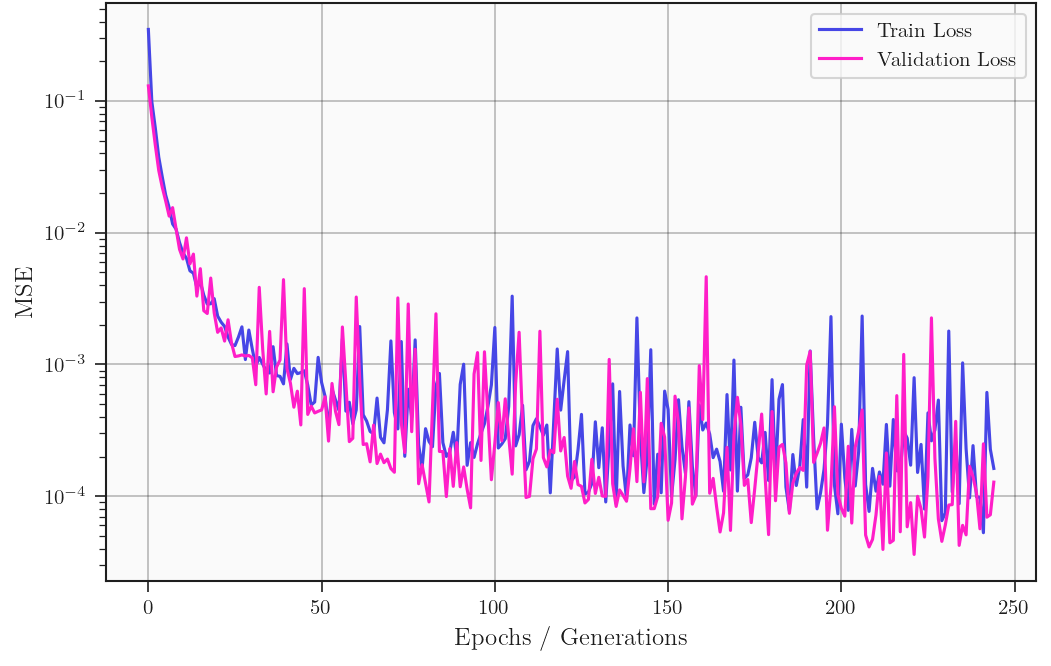
\includegraphics[width=0.8\textwidth]{figures/coul_MLP.png}
    \caption{Curvas de pérdidas de entrenamiento (azul) y validación (violeta) para la MLP Estándar sobre el conjunto de datos correspondiente a la Ley de Coulomb sin ruido.}
    \label{fig:coul_MLP}
\end{figure}

\begin{figure}[H]
    \centering
    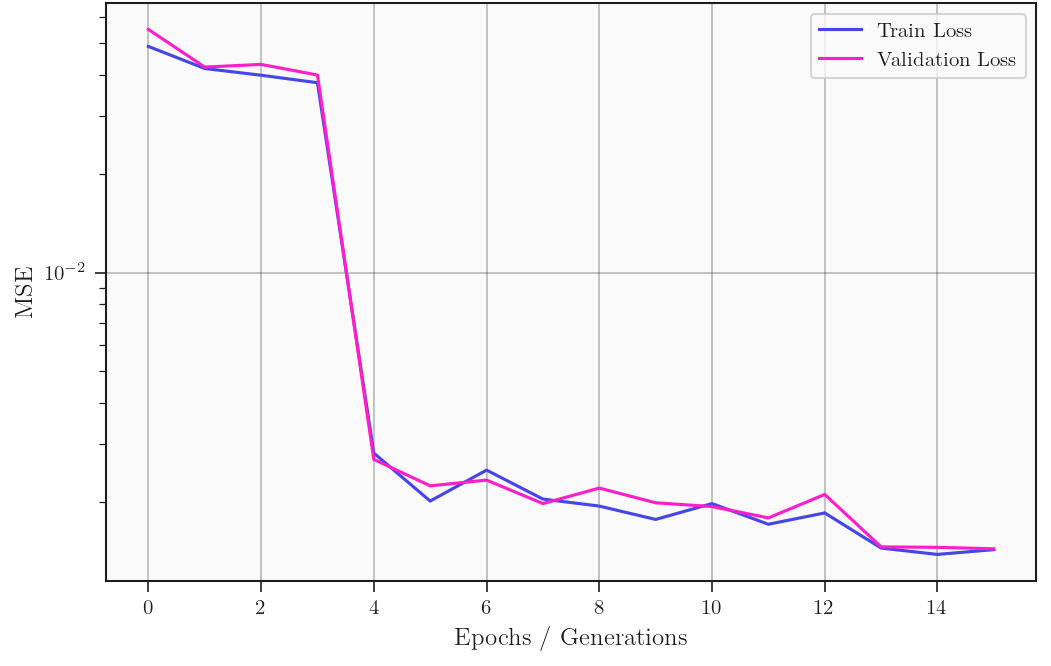
\includegraphics[width=0.8\textwidth]{figures/coul_QLattice.png}
    \caption{Curvas de pérdidas de entrenamiento (azul) y validación (violeta) para el modelo QLattice sobre el conjunto de datos correspondiente a la Ley de Coulomb sin ruido.}
    \label{fig:coul_QLattice}
\end{figure}


El comportamiento de las curvas de las \cref{fig:coul_MLP,fig:coul_QLattice} es similar a la mayoría de gráficas almacenadas en \href{https://github.com/JorgeAcebes/symbolic-physics-discovery/blob/main/results/all_models/gallery_loss.png}{GitHub}: una caída fuertemente marcada en el valor del MSE durante las primeras iteraciones, para después presentar un decrecimiento menos acentuado junto con pequeñas fluctuaciones estocásticas. Es especialmente relevante que en ninguna de las gráficas obtenidas se observa un crecimiento de la curva de validación a la vez que decrece la curva de entrenamiento, confirmando que ninguno de los modelos está sobreajustando a los datos de entrenamiento.



En las \cref{tab:coulomb,tab:oscillator,tab:kepler,tab:idealgas,tab:projectile,tab:timedilation,tab:radioactive,tab:newtoncooling,tab:boltzmann} se resume el desempeño de los modelos ante datos de los sistemas físicos recogidos en la Tabla \ref{tab:Leyes_Fisicas}, evaluados tanto dentro del dominio de entrenamiento (\textit{Inside of Domain}, IOD) como fuera de él (\textit{Outside of Domain}, OOD). Para cada nivel de ruido se reporta el error cuadrático medio (MSE) en ambas condiciones, permitiendo contrastar la capacidad de generalización e interpolación de cada enfoque. Cabe mencionar que se emplea notación e (científica) para aumentar y simplificar la legibilidad y comparación.



\FloatBarrier  
% =========================================================
% TABLE 1: COULOMB'S LAW
% =========================================================
\begin{table}[H]
\centering
\footnotesize
\setlength{\tabcolsep}{0pt}
\makebox[\textwidth][c]{
\begin{tabular}{l @{\hspace{8pt}} c@{\hspace{6pt}}c @{\hspace{12pt}} c@{\hspace{6pt}}c @{\hspace{12pt}} c@{\hspace{6pt}}c}
\toprule
& \multicolumn{2}{c}{\textbf{Sin Ruido}} & \multicolumn{2}{c}{\textbf{Ruido Bajo}} & \multicolumn{2}{c}{\textbf{Ruido Alto}} \\
\cmidrule(lr){2-3}\cmidrule(lr){4-5}\cmidrule(l){6-7}
\textbf{Modelo} & \textbf{MSE$_\text{IOD}$} & \textbf{MSE$_\text{OOD}$} & \textbf{MSE$_\text{IOD}$} & \textbf{MSE$_\text{OOD}$} & \textbf{MSE$_\text{IOD}$} & \textbf{MSE$_\text{OOD}$} \\
\midrule
MLP Estándar & 2.03e-4 & 5.06e-1 & 3.21e-4 & 8.84e-1 & 1.89e-2 & 2.18e-1 \\
MLP Disperso & 7.16e-4 & 7.94e-1 & 7.11e-4 & 9.51e-1 & 1.87e-2 & 7.84e-1 \\
MLP Dropout  & 8.97e-3 & 9.59e-1 & 6.70e-3 & 9.31e-1 & 4.28e-2 & 1.04e+0 \\
\midrule
Polinómico   & 6.54e-3 & 5.32e+6 & 6.64e-3 & 5.46e+6 & 2.37e-2 & 5.18e+6 \\
PySINDy      & 3.79e-2 & 4.03e+4 & 3.81e-2 & 4.05e+4 & 5.41e-2 & 3.59e+4 \\
GPLearn      & 3.01e-13 & 0.00e+0 & 1.76e-4 & 0.00e+0 & 1.72e-2 & 0.00e+0 \\
PySR         & 3.14e-13 & 0.00e+0 & 1.76e-4 & 0.00e+0 & 1.72e-2 & 0.00e+0 \\
QLattice     & 1.42e-3 & 3.96e-1 & 2.72e-4 & 1.67e-6 & 1.80e-2 & 3.03e-3 \\
\bottomrule
\end{tabular}
}
\caption{Resultados para la \textbf{Ley de Coulomb} ($F = q_1 q_2 / r^2$).}
\label{tab:coulomb}
\end{table}

% =========================================================
% TABLE 2: HARMONIC OSCILLATOR
% =========================================================
\begin{table}[H]
\centering
\footnotesize
\setlength{\tabcolsep}{0pt}
\makebox[\textwidth][c]{
\begin{tabular}{l @{\hspace{8pt}} c@{\hspace{6pt}}c @{\hspace{12pt}} c@{\hspace{6pt}}c @{\hspace{12pt}} c@{\hspace{6pt}}c}
\toprule
& \multicolumn{2}{c}{\textbf{Sin Ruido}} & \multicolumn{2}{c}{\textbf{Ruido Bajo}} & \multicolumn{2}{c}{\textbf{Ruido Alto}} \\
\cmidrule(lr){2-3}\cmidrule(lr){4-5}\cmidrule(l){6-7}
\textbf{Modelo} & \textbf{MSE$_\text{IOD}$} & \textbf{MSE$_\text{OOD}$} & \textbf{MSE$_\text{IOD}$} & \textbf{MSE$_\text{OOD}$} & \textbf{MSE$_\text{IOD}$} & \textbf{MSE$_\text{OOD}$} \\
\midrule
MLP Estándar & 4.09e-9  & 1.19e-3 & 1.60e-4 & 7.57e-3 & 1.41e-2 & 1.73e-4 \\
MLP Disperso & 2.23e-5  & 3.08e+0 & 1.99e-4 & 3.14e+0 & 1.42e-2 & 5.89e+0 \\
MLP Dropout  & 1.36e-3  & 3.79e-2 & 3.45e-3 & 1.11e-1 & 1.70e-2 & 5.90e-2 \\
\midrule
Polinómico   & 8.37e-14 & 5.01e-7 & 1.42e-4 & 9.37e+0 & 1.41e-2 & 2.03e+2 \\
PySINDy      & 1.92e-14 & 3.01e-13 & 1.42e-4 & 2.95e-9 & 1.40e-2 & 1.27e-5 \\
GPLearn      & 3.51e-5  & 5.30e-4 & 1.81e-4 & 5.30e-4 & 1.41e-2 & 5.30e-4 \\
PySR         & 0.00e+0  & 0.00e+0 & 1.42e-4 & 6.30e-8 & 1.41e-2 & 3.65e-6 \\
QLattice     & 5.37e-15 & \text{N/D} & 1.45e-4 & 2.36e-6 & 1.43e-2 & 7.47e-4 \\
\bottomrule
\end{tabular}
}
\caption{Resultados para el \textbf{Oscilador Armónico} ($F = -x$).}
\label{tab:oscillator}
\end{table}

% =========================================================
% TABLE 3: KEPLER'S THIRD LAW
% =========================================================
\begin{table}[H]
\centering
\footnotesize
\setlength{\tabcolsep}{0pt}
\makebox[\textwidth][c]{
\begin{tabular}{l @{\hspace{8pt}} c@{\hspace{6pt}}c @{\hspace{12pt}} c@{\hspace{6pt}}c @{\hspace{12pt}} c@{\hspace{6pt}}c}
\toprule
& \multicolumn{2}{c}{\textbf{Sin Ruido}} & \multicolumn{2}{c}{\textbf{Ruido Bajo}} & \multicolumn{2}{c}{\textbf{Ruido Alto}} \\
\cmidrule(lr){2-3}\cmidrule(lr){4-5}\cmidrule(l){6-7}
\textbf{Modelo} & \textbf{MSE$_\text{IOD}$} & \textbf{MSE$_\text{OOD}$} & \textbf{MSE$_\text{IOD}$} & \textbf{MSE$_\text{OOD}$} & \textbf{MSE$_\text{IOD}$} & \textbf{MSE$_\text{OOD}$} \\
\midrule
MLP Estándar & 2.01e-6 & 1.00e+2 & 2.48e-4 & 9.33e+1 & 2.45e-2 & 9.10e+1 \\
MLP Disperso & 3.17e-5 & 3.03e+2 & 2.66e-4 & 3.03e+2 & 2.29e-2 & 3.23e+2 \\
MLP Dropout  & 3.74e-3 & 1.36e+2 & 1.59e-3 & 1.09e+2 & 2.63e-2 & 1.30e+2 \\
\midrule
Polinómico   & 3.45e-7  & 6.30e+4 & 2.32e-4 & 9.23e+4 & 2.23e-2 & 8.38e+4 \\
PySINDy      & 2.20e-5  & 4.95e+1 & 6.22e-4 & 1.76e+1 & 2.24e-2 & 5.50e+1 \\
GPLearn      & 3.41e-13 & 1.20e-30 & 2.32e-4 & 1.20e-30 & 2.24e-2 & 1.20e-30 \\
PySR         & 4.04e-11 & 1.32e-8 & 2.32e-4 & 4.12e-6 & 2.24e-2 & 5.90e-4 \\
QLattice     & 1.80e-7  & 3.34e-5 & 2.38e-4 & 5.31e-3 & 2.26e-2 & 9.66e-3 \\
\bottomrule
\end{tabular}
}
\caption{Resultados para la \textbf{Tercera Ley de Kepler} ($T = r^{3/2}$).}
\label{tab:kepler}
\end{table}

% =========================================================
% TABLE 4: IDEAL GAS LAW
% =========================================================
\begin{table}[H]
\centering
\footnotesize
\setlength{\tabcolsep}{0pt}
\makebox[\textwidth][c]{
\begin{tabular}{l @{\hspace{8pt}} c@{\hspace{6pt}}c @{\hspace{12pt}} c@{\hspace{6pt}}c @{\hspace{12pt}} c@{\hspace{6pt}}c}
\toprule
& \multicolumn{2}{c}{\textbf{Sin Ruido}} & \multicolumn{2}{c}{\textbf{Ruido Bajo}} & \multicolumn{2}{c}{\textbf{Ruido Alto}} \\
\cmidrule(lr){2-3}\cmidrule(lr){4-5}\cmidrule(l){6-7}
\textbf{Modelo} & \textbf{MSE$_\text{IOD}$} & \textbf{MSE$_\text{OOD}$} & \textbf{MSE$_\text{IOD}$} & \textbf{MSE$_\text{OOD}$} & \textbf{MSE$_\text{IOD}$} & \textbf{MSE$_\text{OOD}$} \\
\midrule
MLP Estándar & 1.81e-5 & 9.21e+0 & 1.13e-4 & 7.91e+0 & 1.01e-2 & 8.73e+0 \\
MLP Disperso & 9.73e-5 & 1.01e+1 & 2.12e-4 & 1.02e+1 & 1.03e-2 & 1.10e+1 \\
MLP Dropout  & 2.25e-3 & 1.23e+1 & 3.05e-3 & 1.06e+1 & 1.59e-2 & 1.64e+1 \\
\midrule
Polinómico   & 3.15e-5  & 3.29e+3 & 1.27e-4 & 2.85e+3 & 9.83e-3 & 1.69e+3 \\
PySINDy      & 1.76e-3  & 8.91e+3 & 1.69e-3 & 6.25e+3 & 1.15e-2 & 3.39e+3 \\
GPLearn      & 3.21e-13 & 0.00e+0 & 9.35e-5 & 0.00e+0 & 9.73e-3 & 0.00e+0 \\
PySR         & 3.21e-13 & 0.00e+0 & 9.35e-5 & 0.00e+0 & 9.73e-3 & 0.00e+0 \\
QLattice     & 1.24e-8  & 6.09e-7 & 3.42e-4 & 1.47e+0 & 1.02e-2 & 2.24e+1 \\
\bottomrule
\end{tabular}
}
\caption{Resultados para la \textbf{Ley de los Gases Ideales} ($P = nT/V$).}
\label{tab:idealgas}
\end{table}

% =========================================================
% TABLE 5: PROJECTILE RANGE
% =========================================================
\begin{table}[H]
\centering
\footnotesize
\setlength{\tabcolsep}{0pt}
\makebox[\textwidth][c]{
\begin{tabular}{l @{\hspace{8pt}} c@{\hspace{6pt}}c @{\hspace{12pt}} c@{\hspace{6pt}}c @{\hspace{12pt}} c@{\hspace{6pt}}c}
\toprule
& \multicolumn{2}{c}{\textbf{Sin Ruido}} & \multicolumn{2}{c}{\textbf{Ruido Bajo}} & \multicolumn{2}{c}{\textbf{Ruido Alto}} \\
\cmidrule(lr){2-3}\cmidrule(lr){4-5}\cmidrule(l){6-7}
\textbf{Modelo} & \textbf{MSE$_\text{IOD}$} & \textbf{MSE$_\text{OOD}$} & \textbf{MSE$_\text{IOD}$} & \textbf{MSE$_\text{OOD}$} & \textbf{MSE$_\text{IOD}$} & \textbf{MSE$_\text{OOD}$} \\
\midrule
MLP Estándar & 5.52e-5 & 1.24e+3 & 6.15e-4 & 1.33e+3 & 5.00e-2 & 1.42e+3 \\
MLP Disperso & 2.79e-4 & 1.57e+3 & 7.81e-4 & 1.60e+3 & 4.89e-2 & 1.62e+3 \\
MLP Dropout  & 1.43e-2 & 1.61e+3 & 1.33e-2 & 1.59e+3 & 6.31e-2 & 1.42e+3 \\
\midrule
Polinómico   & 2.41e-5  & 1.21e+3 & 5.00e-4 & 2.02e+3 & 4.81e-2 & 1.71e+3 \\
PySINDy      & 9.44e-4  & 3.21e-1 & 1.43e-3 & 3.28e-1 & 5.04e-2 & 1.16e+1 \\
GPLearn      & 4.41e-1  & \text{N/D} & 4.41e-1 & \text{N/D} & 4.92e-1 & \text{N/D} \\
PySR         & 2.14e-12 & 0.00e+0 & 4.71e-4 & 0.00e+0 & 4.79e-2 & 1.87e-3 \\
QLattice     & 3.97e-4  & 1.22e+3 & 2.45e-3 & 1.70e+3 & 4.98e-2 & 3.93e-1 \\
\bottomrule
\end{tabular}
}
\caption{Resultados para el \textbf{Alcance del Proyectil} ($R = v_0^2 \sin(2\theta)$).}
\label{tab:projectile}
\end{table}

% =========================================================
% TABLE 6: TIME DILATION
% =========================================================
\begin{table}[H]
\centering
\footnotesize
\setlength{\tabcolsep}{0pt}
\makebox[\textwidth][c]{
\begin{tabular}{l @{\hspace{8pt}} c@{\hspace{6pt}}c @{\hspace{12pt}} c@{\hspace{6pt}}c @{\hspace{12pt}} c@{\hspace{6pt}}c}
\toprule
& \multicolumn{2}{c}{\textbf{Sin Ruido}} & \multicolumn{2}{c}{\textbf{Ruido Bajo}} & \multicolumn{2}{c}{\textbf{Ruido Alto}} \\
\cmidrule(lr){2-3}\cmidrule(lr){4-5}\cmidrule(l){6-7}
\textbf{Modelo} & \textbf{MSE$_\text{IOD}$} & \textbf{MSE$_\text{OOD}$} & \textbf{MSE$_\text{IOD}$} & \textbf{MSE$_\text{OOD}$} & \textbf{MSE$_\text{IOD}$} & \textbf{MSE$_\text{OOD}$} \\
\midrule
MLP Estándar & 3.00e-5 & 7.91e+2 & 1.15e-4 & 8.05e+2 & 7.11e-3 & 7.83e+2 \\
MLP Disperso & 5.76e-5 & 8.13e+2 & 1.30e-4 & 8.14e+2 & 7.04e-3 & 8.39e+2 \\
MLP Dropout  & 2.22e-3 & 7.90e+2 & 3.17e-3 & 7.95e+2 & 9.49e-3 & 7.84e+2 \\
\midrule
Polinómico   & 1.62e-3 & 5.83e+2 & 1.70e-3 & 5.41e+2 & 8.38e-3 & 3.46e+3 \\
PySINDy      & 1.01e-2 & 2.62e+2 & 1.02e-2 & 2.63e+2 & 1.72e-2 & 2.61e+2 \\
GPLearn      & 1.64e-1 & 5.78e+2 & 1.64e-1 & 5.78e+2 & 1.71e-1 & 5.78e+2 \\
PySR         & 1.48e-4 & 2.34e+2 & 1.25e-4 & \text{N/D} & 8.92e-3 & 2.85e+2 \\
QLattice     & 1.52e-4 & 1.92e+2 & 2.04e-4 & 1.89e+2 & 6.88e-3 & 1.92e+2 \\
\bottomrule
\end{tabular}
}
\caption{Resultados para la \textbf{Dilatación del Tiempo} ($t' = t/\sqrt{1-v^2}$).}
\label{tab:timedilation}
\end{table}

% =========================================================
% TABLE 7: RADIOACTIVE DECAY
% =========================================================
\begin{table}[H]
\centering
\footnotesize
\setlength{\tabcolsep}{0pt}
\makebox[\textwidth][c]{
\begin{tabular}{l @{\hspace{8pt}} c@{\hspace{6pt}}c @{\hspace{12pt}} c@{\hspace{6pt}}c @{\hspace{12pt}} c@{\hspace{6pt}}c}
\toprule
& \multicolumn{2}{c}{\textbf{Sin Ruido}} & \multicolumn{2}{c}{\textbf{Ruido Bajo}} & \multicolumn{2}{c}{\textbf{Ruido Alto}} \\
\cmidrule(lr){2-3}\cmidrule(lr){4-5}\cmidrule(l){6-7}
\textbf{Modelo} & \textbf{MSE$_\text{IOD}$} & \textbf{MSE$_\text{OOD}$} & \textbf{MSE$_\text{IOD}$} & \textbf{MSE$_\text{OOD}$} & \textbf{MSE$_\text{IOD}$} & \textbf{MSE$_\text{OOD}$} \\
\midrule
MLP Estándar & 9.74e-7 & 4.84e+0 & 1.19e-5 & 3.15e+0 & 9.12e-4 & 4.64e+0 \\
MLP Disperso & 1.70e-5 & 1.58e+0 & 1.61e-5 & 1.54e+0 & 8.88e-4 & 1.56e+0 \\
MLP Dropout  & 3.12e-4 & 4.87e+0 & 1.48e-4 & 4.12e+0 & 1.05e-3 & 3.96e+0 \\
\midrule
Polinómico   & 9.21e-6  & 4.88e+3 & 1.78e-5 & 5.34e+3 & 8.77e-4 & 5.09e+3 \\
PySINDy      & 1.97e-4  & 5.10e+2 & 2.05e-4 & 5.14e+2 & 1.06e-3 & 5.30e+2 \\
GPLearn      & 5.85e-2  & 2.87e-1 & 5.85e-2 & 2.87e-1 & 5.92e-2 & 2.87e-1 \\
PySR         & 4.70e-15 & 0.00e+0 & 8.55e-6 & 0.00e+0 & 8.60e-4 & 0.00e+0 \\
QLattice     & 1.48e-12 & 1.78e-13 & 8.70e-6 & 7.76e-8 & 8.61e-4 & 3.45e-7 \\
\bottomrule
\end{tabular}
}
\caption{Resultados para la \textbf{Desintegración Radiactiva} ($N = e^{-\lambda t}$).}
\label{tab:radioactive}
\end{table}

% =========================================================
% TABLE 8: NEWTON'S COOLING LAW
% =========================================================
\begin{table}[H]
\centering
\footnotesize
\setlength{\tabcolsep}{0pt}
\makebox[\textwidth][c]{
\begin{tabular}{l @{\hspace{8pt}} c@{\hspace{6pt}}c @{\hspace{12pt}} c@{\hspace{6pt}}c @{\hspace{12pt}} c@{\hspace{6pt}}c}
\toprule
& \multicolumn{2}{c}{\textbf{Sin Ruido}} & \multicolumn{2}{c}{\textbf{Ruido Bajo}} & \multicolumn{2}{c}{\textbf{Ruido Alto}} \\
\cmidrule(lr){2-3}\cmidrule(lr){4-5}\cmidrule(l){6-7}
\textbf{Modelo} & \textbf{MSE$_\text{IOD}$} & \textbf{MSE$_\text{OOD}$} & \textbf{MSE$_\text{IOD}$} & \textbf{MSE$_\text{OOD}$} & \textbf{MSE$_\text{IOD}$} & \textbf{MSE$_\text{OOD}$} \\
\midrule
MLP Estándar & 2.93e-7 & 1.28e+1 & 1.61e-5 & 7.39e+0 & 9.72e-4 & 1.02e+1 \\
MLP Disperso & 9.82e-6 & 4.86e+0 & 1.99e-5 & 4.95e+0 & 9.83e-4 & 4.99e+0 \\
MLP Dropout  & 1.41e-4 & 8.92e+0 & 1.38e-4 & 8.68e+0 & 1.36e-3 & 9.78e+0 \\
\midrule
Polinómico   & 9.55e-6  & 3.14e+3 & 1.83e-5 & 2.50e+3 & 9.55e-4 & 5.45e+3 \\
PySINDy      & 2.01e-4  & 2.65e+2 & 2.07e-4 & 2.67e+2 & 1.18e-3 & 5.61e+2 \\
GPLearn      & 9.13e-2  & 1.34e-1 & 9.13e-2 & 1.34e-1 & 9.21e-2 & 1.34e-1 \\
PySR         & 8.78e-14 & 0.00e+0 & 8.76e-6 & 1.46e-8 & 9.44e-4 & 7.29e-12 \\
QLattice     & 6.22e-10 & 1.81e-16 & 9.27e-6 & 4.71e-16 & 9.43e-4 & 4.90e-7 \\
\bottomrule
\end{tabular}
}
\caption{Resultados para la \textbf{Ley del Enfriamiento de Newton} ($T = 1 + e^{-kt}$).}
\label{tab:newtoncooling}
\end{table}

% =========================================================
% TABLE 9: BOLTZMANN ENTROPY
% =========================================================
\begin{table}[H]
\centering
\footnotesize
\setlength{\tabcolsep}{0pt}
\makebox[\textwidth][c]{
\begin{tabular}{l @{\hspace{8pt}} c@{\hspace{6pt}}c @{\hspace{12pt}} c@{\hspace{6pt}}c @{\hspace{12pt}} c@{\hspace{6pt}}c}
\toprule
& \multicolumn{2}{c}{\textbf{Sin Ruido}} & \multicolumn{2}{c}{\textbf{Ruido Bajo}} & \multicolumn{2}{c}{\textbf{Ruido Alto}} \\
\cmidrule(lr){2-3}\cmidrule(lr){4-5}\cmidrule(l){6-7}
\textbf{Modelo} & \textbf{MSE$_\text{IOD}$} & \textbf{MSE$_\text{OOD}$} & \textbf{MSE$_\text{IOD}$} & \textbf{MSE$_\text{OOD}$} & \textbf{MSE$_\text{IOD}$} & \textbf{MSE$_\text{OOD}$} \\
\midrule
MLP Estándar & 9.67e-7 & 2.71e+3 & 5.47e-5 & 4.17e+2 & 3.53e-3 & 4.18e+3 \\
MLP Disperso & 9.19e-6 & 3.02e+0 & 4.60e-5 & 1.38e+0 & 3.52e-3 & 1.56e+0 \\
MLP Dropout  & 3.68e-4 & 6.65e+2 & 2.63e-4 & 9.09e+2 & 3.88e-3 & 8.20e+2 \\
\midrule
Polinómico   & 1.49e-5  & 1.41e+17 & 4.96e-5 & 1.40e+17 & 3.53e-3 & 1.11e+17 \\
PySINDy      & 8.55e-5  & 1.17e+1  & 1.23e-4 & 1.16e+1  & 1.47e-2 & 1.24e+2 \\
GPLearn      & 7.95e-14 & 0.00e+0  & 3.48e-5 & 0.00e+0  & 3.50e-3 & 0.00e+0 \\
PySR         & 7.95e-14 & 0.00e+0  & 3.48e-5 & 0.00e+0  & 3.50e-3 & 0.00e+0 \\
QLattice     & 1.08e-12 & 1.25e-8  & 3.56e-5 & 5.29e-6  & 3.52e-3 & 2.66e-4 \\
\bottomrule
\end{tabular}
}
\caption{Resultados para la \textbf{Entropía de Boltzmann} ($S =\ln\Omega$).}
\label{tab:boltzmann}
\end{table}

De manera general, se observa que en el rango de estudio, IOD, los modelos presentan MSE relativamente bajos, pero este hecho carece de relevancia física si los resultados no pueden extrapolarse a un dominio no estudiado. Por ello, el análisis de la calidad de las ecuaciones ofrecidas por los regresores y el comportamiento de las MLP se ponen a prueba en el dominio OOD. En este contexto, se produce una clara dominancia de los regresores simbólicos, particularmente de PySR, GPLearn y QLattice, los cuales promedian un MSE fuera del dominio de entrenamiento muy inferior respecto al resto de modelos.

Estos resultados se muestran de manera más visual a continuación. En las \cref{fig:kepler_ood,fig:oscillator_ood} se presentan gráficos de barras con el MSE para cada modelo y nivel de ruido, relativas a los datos de la Ley de Kepler y el oscilador armónico, para muestras fuera del rango de entrenamiento. La bondad de la predicción se clasifica según el criterio establecido en la Sección \ref{subsec:eval}: exacta, precisa, aproximada e incorrecta. Asimismo, el resto de gráficos de barras correspondientes al resto de leyes físicas se encuentran en \href{https://github.com/JorgeAcebes/symbolic-physics-discovery/tree/main/results/results_ood}{GitHub} \cite{repositorio}.

Si bien estos gráficos de barras permiten un análisis detallado, es complejo dilucidar una conclusión clara de manera general. Por ello, se condensa la información en la Figura \ref{fig:model_recovery}, obviando los valores particulares del MSE para cada modelo y mostrando exclusivamente la clasificación por categoría. 



\begin{figure}[H]
    \centering
    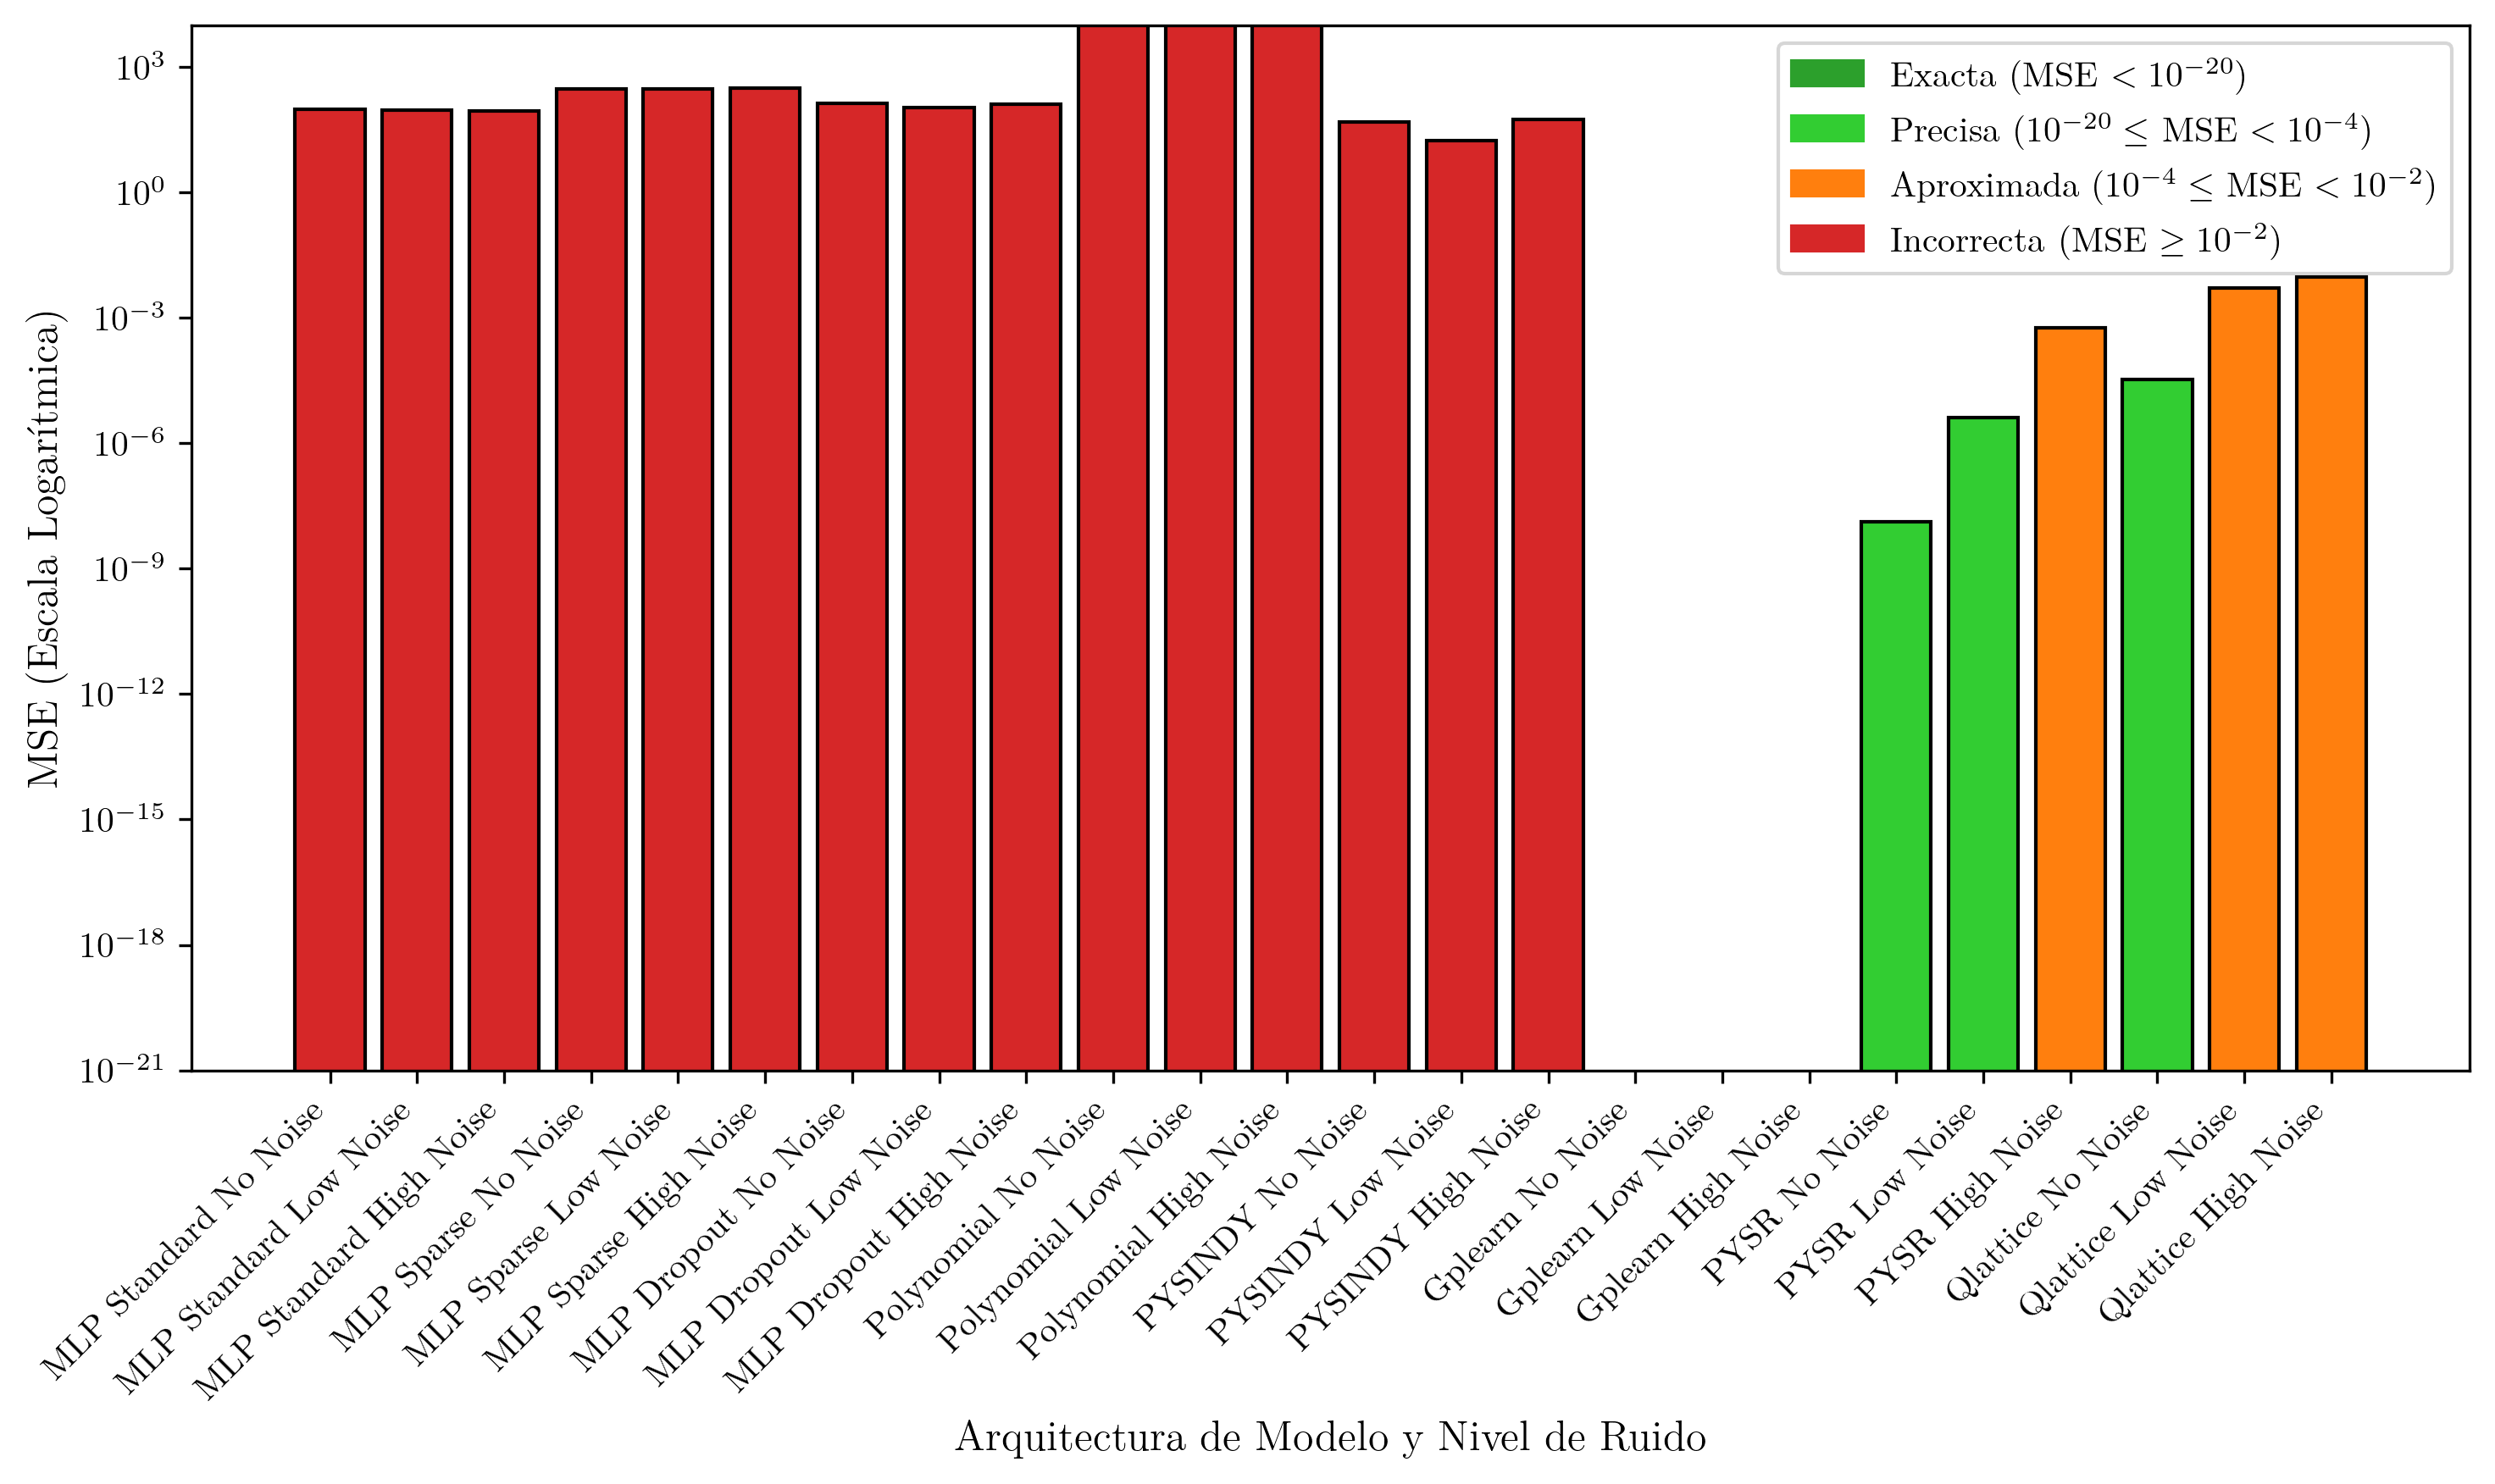
\includegraphics[width=0.95\textwidth]{figures/kepler_mse_ood.png}
    \caption{Gráfico de barras con el MSE para cada modelo y nivel de ruido con código de color para la bondad de la predicción (verde oscuro: exacta, verde: precisa, naranja: aproximada, rojo: incorrecta) relativa a los datos de la \textbf{Tercera Ley de Kepler} para muestras fuera del rango de entrenamiento (OOD).}
    \label{fig:kepler_ood}
\end{figure}

\begin{figure}[H]
    \centering
    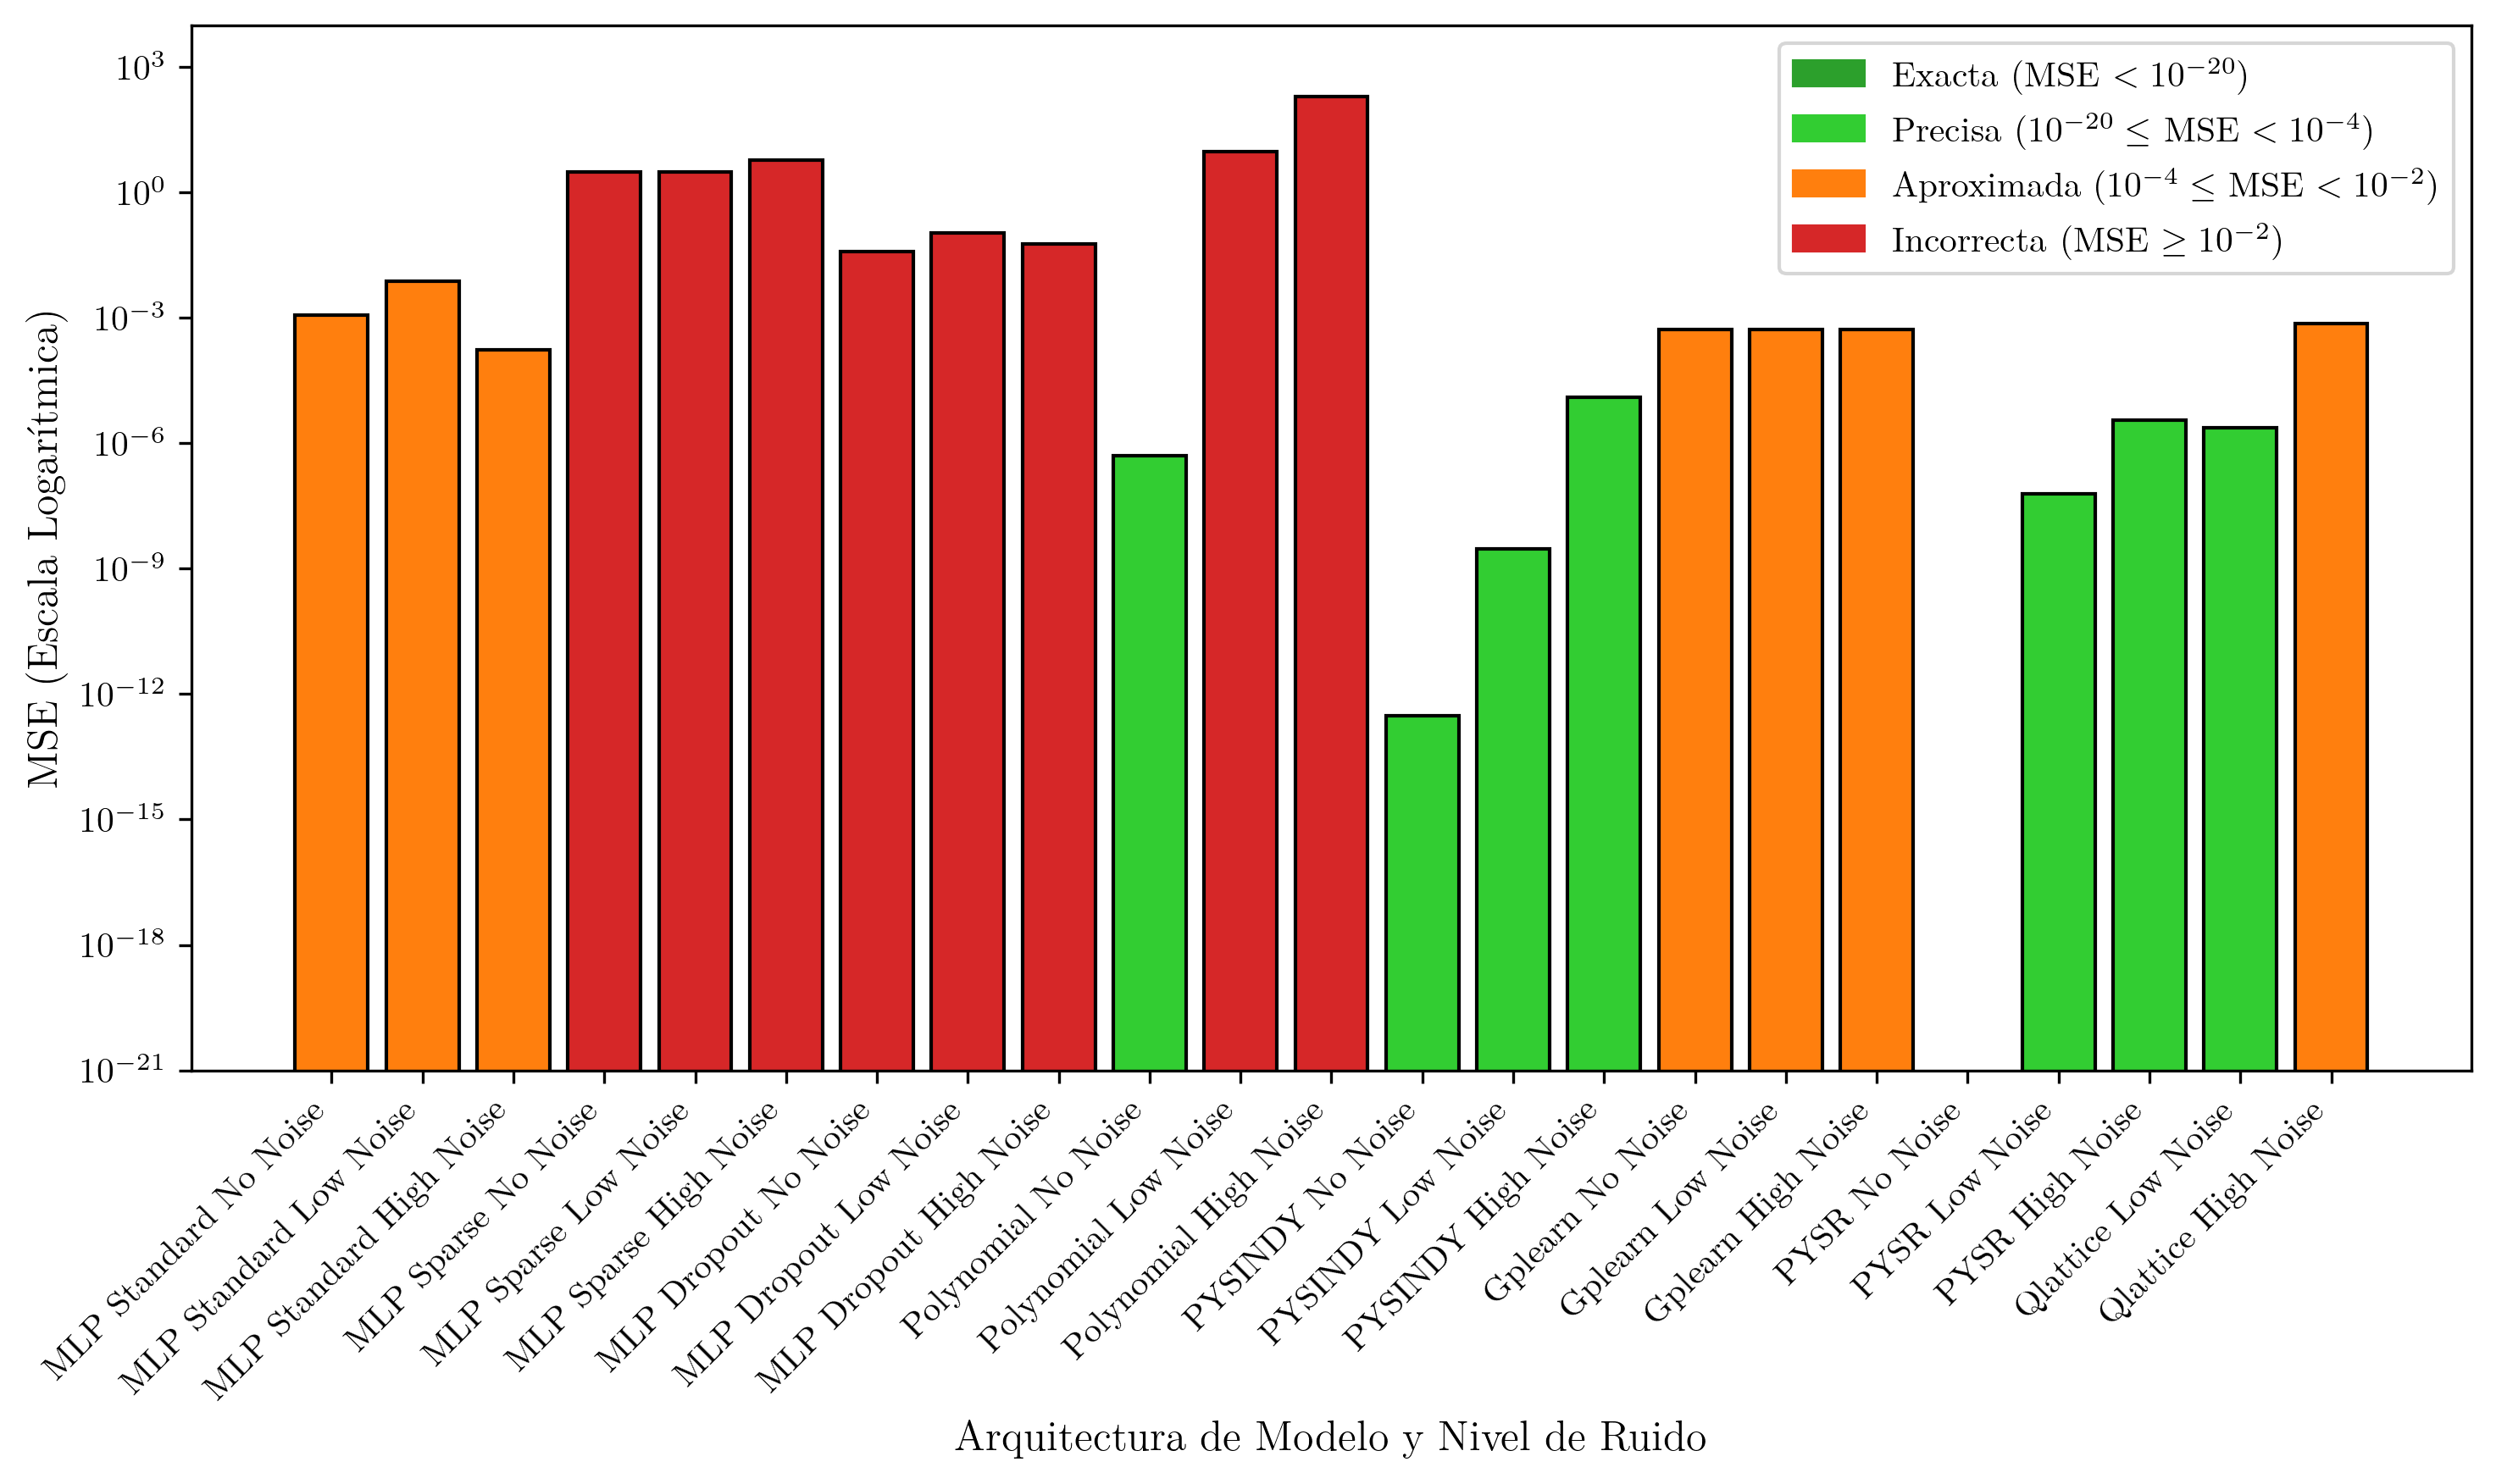
\includegraphics[width=0.95\textwidth]{figures/oscillator_mse_ood.png}
    \caption{Gráfico de barras con el MSE para cada modelo y nivel de ruido con código de color para la bondad de la predicción (verde oscuro: exacta, verde: precisa, naranja: aproximada, rojo: incorrecta) relativa a los datos del \textbf{Oscilador Armónico} para muestras fuera del rango de entrenamiento (OOD).}
    \label{fig:oscillator_ood}
\end{figure}

\begin{figure}[H]
    \centering
    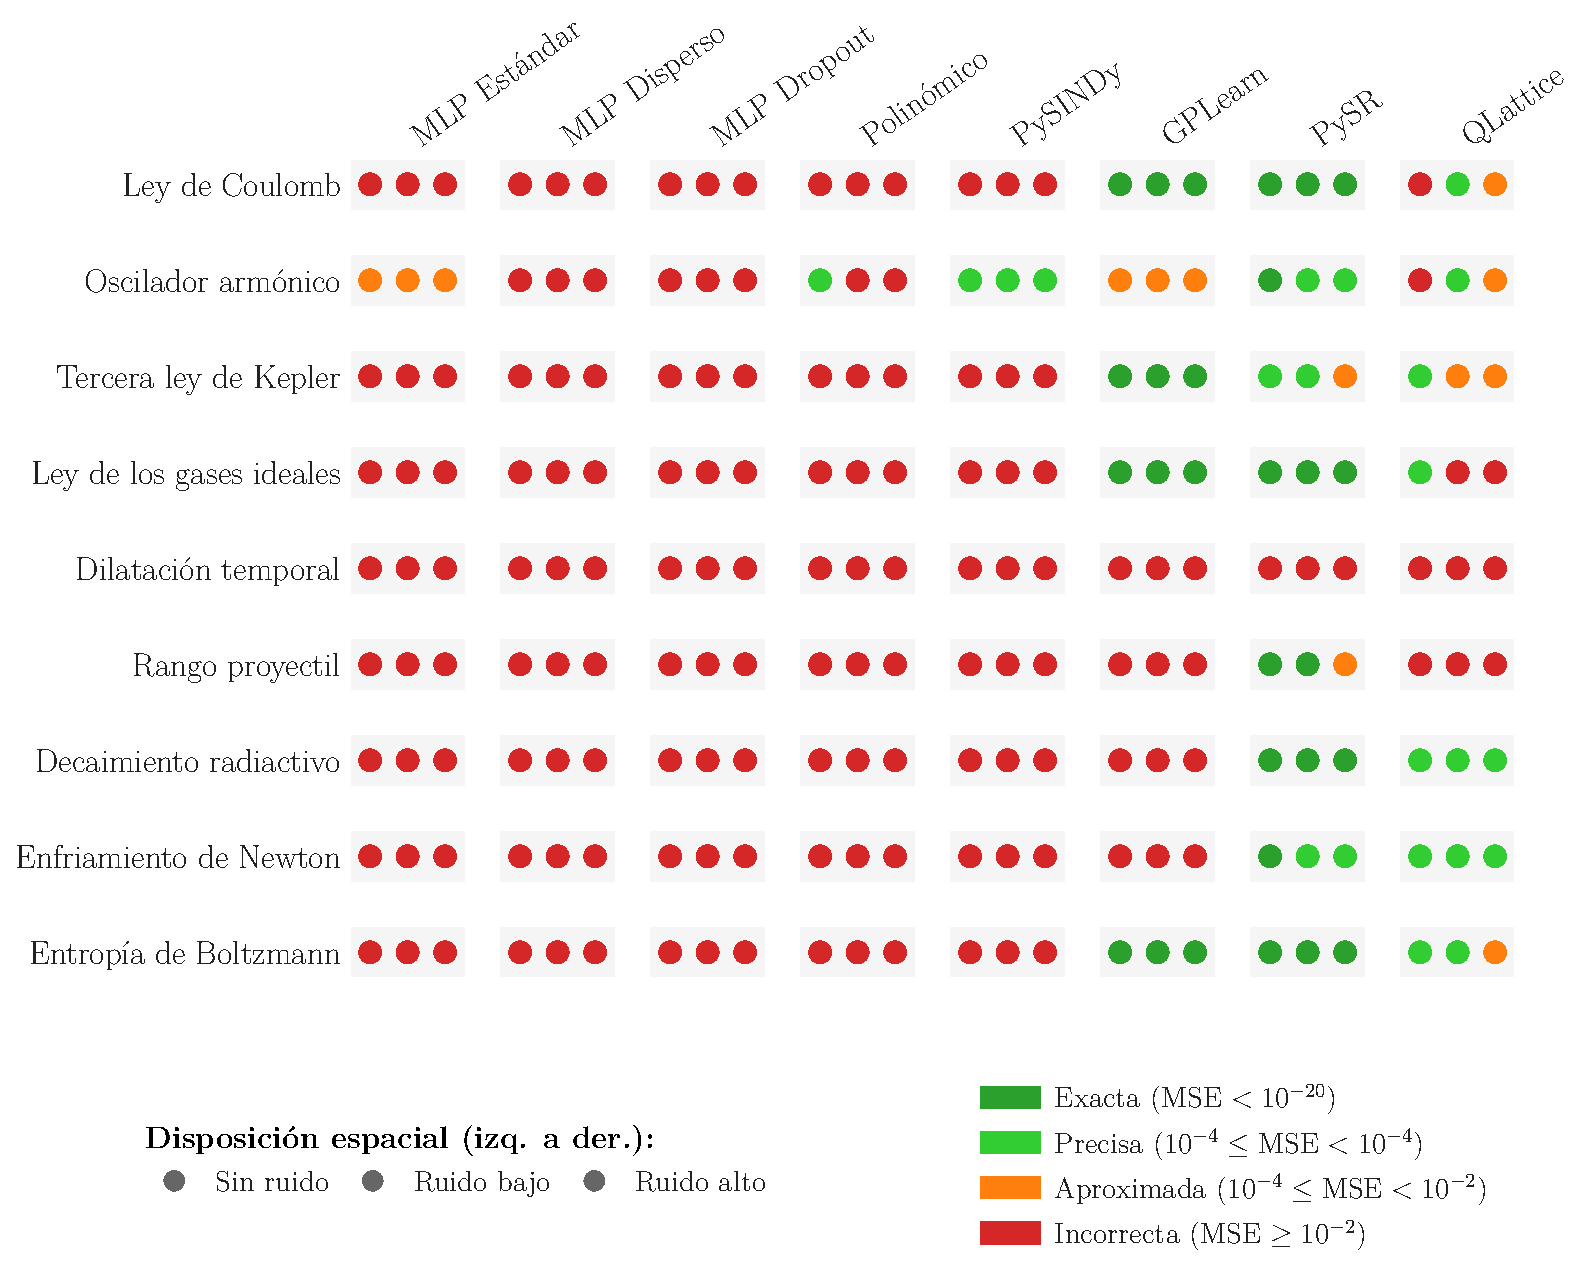
\includegraphics[width=\textwidth]{figures/model_recovery.pdf}
    \caption{Bondad de la predicción de cada modelo para cada nivel de ruido y cada ley para muestras fuera del rango de entrenamiento (OOD).}
    \label{fig:model_recovery}
\end{figure}



Finalmente, la Figura \ref{fig:model_recovery} se desglosa en tres tablas en las \cref{fig:table_no_noise,fig:table_low_noise,fig:table_high_noise}, mostrando no solo la categoría según el MSE, sino también las leyes obtenidas por los regresores. Así se refleja la verdadera ventaja de los regresores simbólicos, los cuales no solo logran unos mejores resultados en términos de MSE, sino que producen expresiones físicamente interpretables.




\begin{figure}[H]
    \centering
    \makebox[\textwidth][c]{%
        \begin{minipage}{1.2\textwidth}
            \centering
            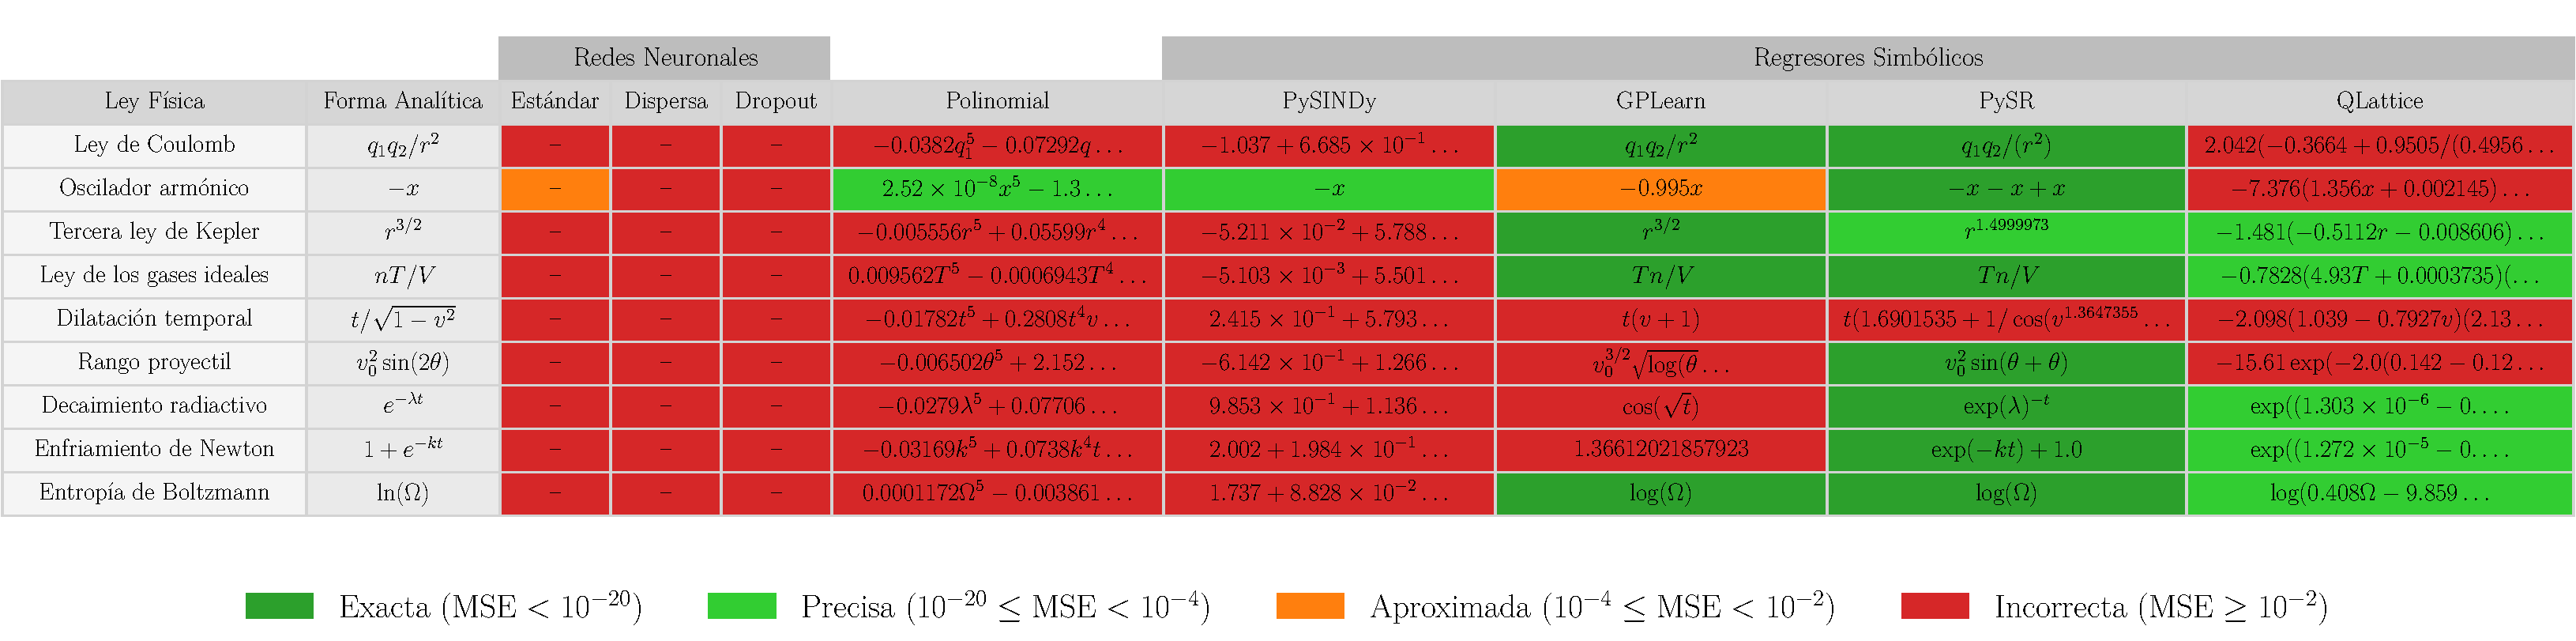
\includegraphics[width=1\textwidth]{figures/table_no_noise.pdf}
        \end{minipage}%
    }
    \caption{Tabla comparativa de las expresiones matemáticas recuperadas por los regresores simbólicos y el {MSE$_\text{OOD}$} para cada modelo para datos sin ruido.}
    \label{fig:table_no_noise}
\end{figure}


\begin{figure}[H]
    \centering
    \makebox[\textwidth][c]{%
        \begin{minipage}{1.2\textwidth}
            \centering
            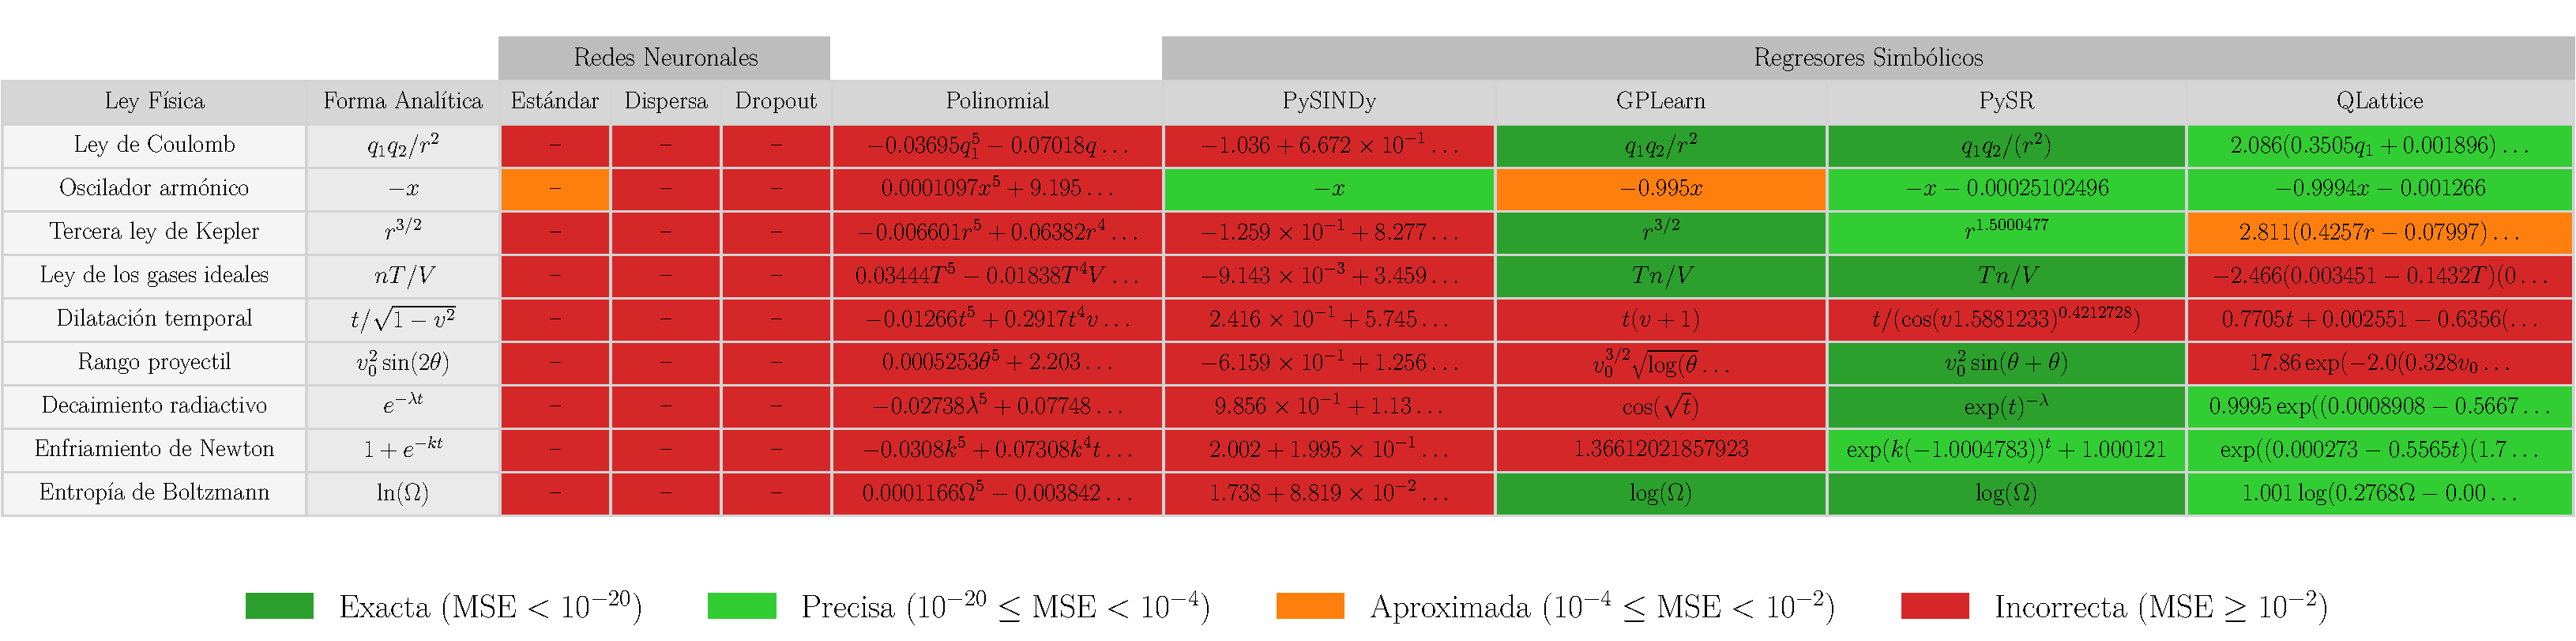
\includegraphics[width=1\textwidth]{figures/table_low_noise.pdf}
        \end{minipage}%
    }
    \caption{Tabla comparativa de las expresiones matemáticas recuperadas por los regresores simbólicos y el {MSE$_\text{OOD}$} para cada modelo para datos con ruido bajo.}
    \label{fig:table_low_noise}

\end{figure}

\begin{figure}[H]
    \centering
    \makebox[\textwidth][c]{%
        \begin{minipage}{1.2\textwidth}
            \centering
            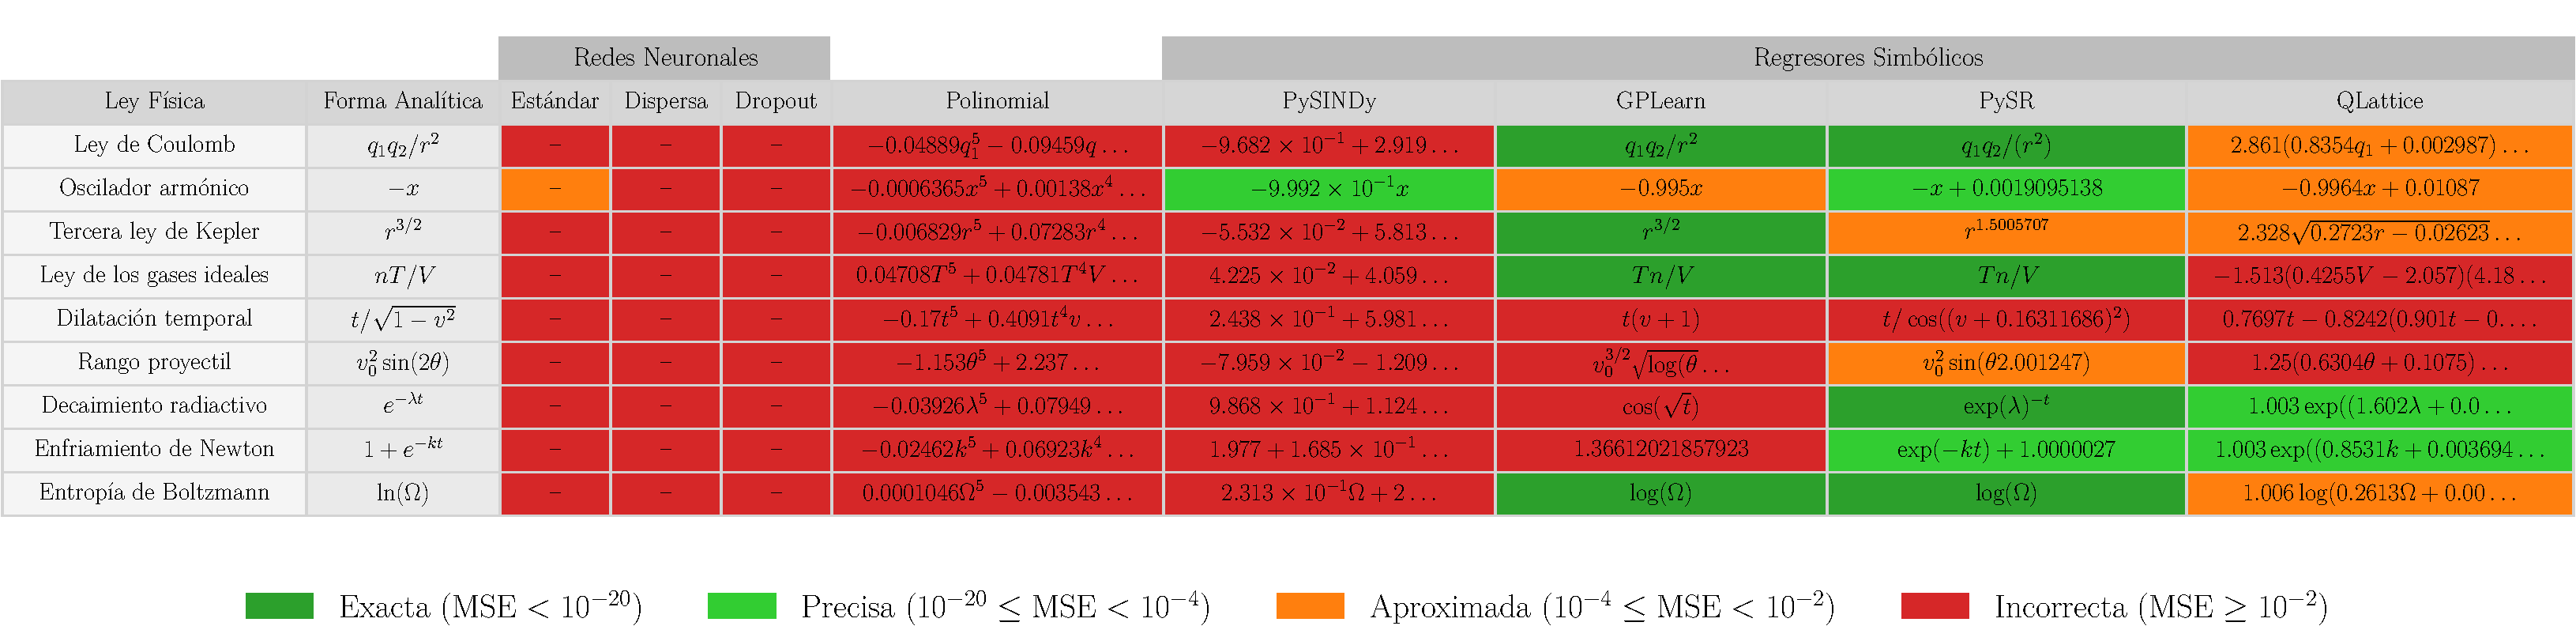
\includegraphics[width=1\textwidth]{figures/table_high_noise.pdf}
        \end{minipage}%
    }
    \caption{Tabla comparativa de las expresiones matemáticas recuperadas por los regresores simbólicos y el {MSE$_\text{OOD}$} para cada modelo para datos con ruido alto.}
    \label{fig:table_high_noise}
\end{figure}



De la figura \ref{fig:model_recovery} en adelante, se observa una clara superioridad de los regresores simbólicos PySR, GPLearn y QLattice sobre el resto de modelos. La razón de este hecho es que son capaces de generar relaciones matemáticas sencillas con diferentes operadores,
al contrario que las MLP, que no permiten proporcionar expresión matemática alguna, y no únicamente polinomios, como PySINDy y el regresor polinomial. Además, al contar con limitaciones de complejidad intrínsecas en sus funciones de pérdida, el espacio de soluciones se restringe a expresiones compactas y evita el sobreajuste a patrones locales del conjunto de entrenamiento. Así, especialmente GPLearn y PySR respetan el principio de parsimonia, particularmente relevante en casos con ruido, y extrapolan su extraordinario rendimiento en datos IOD a los datos OOD.

Antes de entrar en la discusión detallada de los resultados, es necesario analizar cómo el espacio de operadores disponible en cada algoritmo determina su rendimiento. Aunque excluir funciones no lineales simplificaría el análisis, reduciría drásticamente el alcance físico del estudio, ya que la mayoría de las leyes de la naturaleza involucran relaciones sinusoidales, exponenciales o logarítmicas. Por ello, se han definido previamente los operadores permitidos en cada modelo. Esta restricción estructural se traduce en la incapacidad de GPLearn para reproducir leyes exponenciales y de QLattice para identificar relaciones sinusoidales. Por su parte, los algoritmos de regresión restantes (Regresor Polinomial y PySINDy) presentan una limitación inductiva fundamental: parten de la premisa de que es posible recuperar relaciones matemáticas complejas mediante combinaciones de operaciones simples, lo que genera un sesgo significativo al modelar dinámicas no lineales.

Respecto a las categorías de las \cref{fig:model_recovery,fig:table_no_noise,fig:table_low_noise,fig:table_high_noise}, en primer lugar, la clasificación de ``exacta'' representa casos de éxito en la predicción, observándose exclusivamente en los regresores, muestra de que han logrado obtener las expresiones subyacentes de los datos sintéticos. El modelo que cuenta con más fórmulas exactas es PySR, especialmente en casos sin ruido, aunque consigue reproducir exactamente 4 ecuaciones en caso de ruido alto. Por otro lado, GPLearn también consigue recuperar 4 ecuaciones (curiosamente, el oscilador armónico no es una de ellas), demostrando su superioridad frente al resto de modelos.

En segundo lugar, cuando la predicción se denota como ``precisa'', de nuevo solo logrado por los regresores simbólicos, sugiere que las ecuaciones difieren de la ley física que buscan modelar únicamente en el valor de las constantes. Esto ocurre ocasionalmente en PySR, especialmente en casos con ruido, y en QLattice, el cual parece captar el comportamiento fundamental de las leyes pero sus resultados poseen una complejidad muy alta (gran número de ecuaciones ``precisas'', pero ningún resultado ``exacto''), lo que produce aumentos rápidos del MSE. La mayor complejidad en las ecuaciones de QLattice se debe a su arquitectura probabilística, la cual requiere de un gran número de iteraciones para estabilizarse completamente. A este hecho hay que sumarle que el criterio BIC penaliza la complejidad en función del número de parámetros libres, una métrica que no captura adecuadamente la complejidad topológica de la expresión resultante.

En tercer lugar, la clasificación de ``aproximada'' indica un entendimiento insuficiente de la física subyacente. En particular, cuando una expresión de un regresador simbólico cae en esta categoría, manifiesta que se ha conseguido una fórmula que produce datos cercanos a los reales, pero la forma funcional no es adecuada o contiene constantes que modifican altamente las predicciones. Este tipo de expresiones aparecen especialmente en las obtenidas a partir de datos sintéticos con mucho ruido, para los cuales los modelos pueden tratar de sobreajustar sus términos para obtener mejores MSE en el entrenamiento, resultando en un deterioro en su adecuación general debido a su elevada complejidad.

Por último, si no se ha logrado una predicción con un error relativo medio inferior al 10\%, esta se clasifica como ``incorrecta''. En esta clasificación entran la mayoría de los modelos de perceptrón multicapa, incapaces de aproximar la física para muestras de datos fuera del rango de entrenamiento, independientemente del nivel de ruido, así como la mayoría de predicciones dadas por los modelos de regresión polinómica y PySINDy. La presencia de los regresores simbólicos en esta categoría es causa de la insuficiencia de los términos polinómicos para capturar relaciones multivariables no triviales; sí sirven, en cambio, para casos sencillos. 

Adicionalmente, cabe señalar que ninguno de los modelos consigue reproducir la ecuación de dilatación temporal. Esto ocurre debido a que una gran parte de los puntos estudiados caen en la zona donde $t'\approx t$, y que la ecuación subyacente tiene una alta complejidad, por lo que los modelos no consiguen identificarla. Probablemente, con un mejor condicionamiento de los datos, esto es, para valores de velocidad cercanos a la unidad, los modelos más avanzados serían capaces de extraer la expresión analítica real.

Respecto al análisis de la recuperación de ecuaciones en concreto (\cref{fig:table_no_noise,fig:table_low_noise,fig:table_high_noise}), encontramos varios sucesos dignos de comentar. El primero lo encontramos con la expresión del oscilador armónico, la ecuación más sencilla de todas, que es capaz de ser recuperada por todos los modelos de regresión simbólica salvo por QLattice, no logra converger hacia la solución correcta en el caso sin ruido. Lógicamente, aquellas expresiones con términos exponenciales solo pudieron ser resueltas por los modelos que contenían en su base de operadores la exponencial, a saber: PySR y QLattice. Sin embargo, en cuanto a la expresión con operadores sinusoidales (rango de proyectil), presentes en la base de operadores de PySR y GPLearn, solo es obtenida de manera exacta por el primero de ellos. El último caso reseñable se trata de la fórmula de la entropía de Boltzmann, para la cual, tanto PySR como GPLearn son capaces de recuperar la ecuación exacta, mientras que QLattice obtiene la forma logarítmica pero no su argumento, no obstante, como el logaritmo crece lentamente, su MSE no se dispara al evaluarlo en un rango no muy alejado del original.

Finalmente, evaluamos la robustez de los modelos frente a distintos niveles de ruido. La introducción de ruido leve reduce la convergencia hacia expresiones analíticas exactas. De forma antiintuitiva, esta perturbación beneficia la búsqueda topológica en QLattice, que logra recuperar la forma funcional de la Ley de Coulomb y del oscilador armónico; sin embargo, sobreajusta la ecuación de los gases ideales al introducir constantes no físicas, lo que dispara el error cuadrático medio. 

Al transicionar a ruido alto, PySR y QLattice sufren una degradación esperada: logran conservar las relaciones algebraicas subyacentes, pero desajustan las constantes de acoplamiento. El resto de modelos resulta insensible a este aumento de ruido dada la deficiencia basal de sus predicciones.

En definitiva: el ruido penaliza fuertemente la precisión paramétrica. No obstante, un algoritmo capaz de deducir la expresión correcta con datos carentes de ruido tiende a preservar dicha estructura analítica frente a perturbaciones estocásticas, limitándose a absorber la varianza en los parámetros libres de la ecuación.


\section{Conclusiones}

En este estudio se ha evaluado la capacidad de inferencia analítica de arquitecturas de perceptrón multicapa (MLP), modelos polinómicos y regresores simbólicos (PySR, QLattice, GPLearn, PySINDy) frente a conjuntos de datos de complejidad composicional creciente y perturbación estocástica variable. Para garantizar la validez del trabajo, se ha asegurado una estricta separación en las particiones de datos, y se ha explorado el espacio de hiperparámetros estocásticamente mediante Optuna.

El análisis del rendimiento en régimen de extrapolación fuera de distribución (OOD) valida empíricamente el principio de parsimonia en el modelado físico. Se demuestra que un aumento no justificado en la complejidad topológica de las expresiones conduce sistemáticamente al sobreajuste, manifestado en una divergencia exponencial del error cuadrático medio (MSE) al evaluar dinámicas fuera del dominio de entrenamiento.

Los resultados establecen una clara jerarquía. Los modelos MLP y de regresión polinómica fracasan en la generalización OOD, demostrando su limitación estructural para deducir relaciones algebraicas globales más allá de aproximaciones locales de los datos. En contraste, los regresores simbólicos exhiben capacidad para identificar la expresión analítica exacta. PySR demuestra la mayor robustez topológica y paramétrica, seguido de GPLearn con una tasa de recuperación moderada. QLattice, si bien logra converger hacia la forma funcional correcta en la mayoría de los casos, tiende a generar un colector de soluciones de dimensionalidad excesiva.

En conclusión, la regresión simbólica representa un cambio de paradigma frente a la opacidad del aprendizaje profundo tradicional. Aunque su escalabilidad requiere de un desarrollo continuo de las heurísticas de búsqueda, métodos como PySR demuestran una capacidad excepcional para automatizar la extracción de leyes físicas invariantes puramente a partir de datos empíricos, independizándose de sesgos teóricos a priori.

\newpage
\bibliography{biblio}

\end{document}
